\documentclass[twoside,a4,12p]{report} %,draft,openright]

\usepackage{epsf,graphicx}
\usepackage{latexsym,amssymb}
\usepackage{setspace,cite}
\usepackage{parskip}
\usepackage{amsmath}
\usepackage{amssymb}
\usepackage{listings}
\usepackage{color}
\usepackage{xcolor}
\usepackage{float}
\usepackage{graphicx}
\usepackage[bookmarks=true,pdfborder={0 0 0}]{hyperref}
\usepackage{subcaption}
\usepackage{tensor}
\usepackage{lscape}
\usepackage[export]{adjustbox}
\usepackage{mdframed}
\usepackage{textcomp}

% for margins left, right top bottom
\usepackage{anysize}
\marginsize{4cm}{2.5cm}{4cm}{4cm}

%\usepackage{draft} %draft option - doesn't put full figures in -
            % useful when editing

%does the headers on the pages - keep in
\usepackage{fancyhdr}

%omitting any of these makes the thesis compile without the omitted
%chapter - good for editing single chapters.
%\includeonly{header,intro,background,appendix}
\providecommand{\e}[1]{\ensuremath{10^{#1}}}
\allowdisplaybreaks%%%
\newcommand\scalemath[2]{\scalebox{#1}{\mbox{\ensuremath{\displaystyle #2}}}}

\begin{document}
\newpage

%Puts page numbering of preamble in roman and of main body of thesis in
%arabic. Also defines how chapters and sections are made
\pagenumbering{arabic}
\setcounter{page}{1} \pagestyle{fancy}
\renewcommand{\chaptermark}[1]{\markboth{\chaptername%
\ \thechapter:\,\ #1}{}}
\renewcommand{\sectionmark}[1]{\markright{\thesection\,\ #1}}

%DEFINES TITLE PAGE, and contains abstract, acknowledgements, etc.
\newpage
\thispagestyle{empty}

% ******* Title page *******
% **************************

\vspace*{2cm}
\begin{center}
{\huge\bf Visual Servoing Using Trifocal Tensor\\} \vspace{2cm} {\large
Marwan Osman\\ }
\vspace{3cm}


\includegraphics[height=0.1\textheight]{figures/inrialogo.jpg}

\includegraphics[height=0.1\textheight]{figures/ublogo.png}

\vspace{1cm}
Supervised by: Fran\c{c}ois Chaumette\\
INRIA Rennes Bretagne Atlantique
\end{center}

\vspace{4cm}
\begin{center}
{\large A Thesis Submitted for the Degree of \\MSc Computer Vision (MsCV) \\\vspace{0.3cm} $\cdot$ 2015 $\cdot$}
\end{center}
\singlespacing

\newpage
\thispagestyle{empty}

%ABSTRACT
\begin{abstract}
Visual servoing is an approach for controlling the motion of a robotic system from visual measurements. Many works have been realized in the past in this area, and is mainly divided into two main categories: Image-based, and Pose-based Visual Servoing. The trifocal tensor is well known in computer vision for tracing geometric information from three images of the same scene. The purpose of this thesis is to design a visual servoing method of a 6-DOF manipulator or robot based on the three-view projective geometry properties. Few studies where conducted on this work but they didn't provide a generic analytical solution for 6-DOF robots. This method differs than the two main visual servoing approaches as the control loop is closed over projective measures, which are the trifocal tensor elements. These projective measures are found directly from images across three views, without explicitly recovering the camera pose or directly closing the loop in the image space. The trifocal tensor geometric model is more robust than the two view geometry models as it involves the information given by a third view, and the set of correspondences obtained is more robust to outliers.

\vspace*{5cm}



\begin{center}
\begin{quote}
\it Nothing of me is original. I am the combined effort of everybody I've ever known.\,\ldots
\end{quote}
\end{center}
\hfill{\small Chuck Palahniuk}

\end{abstract}

\chapter*{Acknowledgments}
%\addcontentsline{toc}{chapter} {\protect\numberline{Acknowledgments\hspace{-96pt}}}

\begin{center}
Many thanks to all my professors and colleagues in the VIBOT/MsCV family for giving me the opportunity of joining this family. To my supervisor Prof. Chaumette for his patience and guidance through all the past months working on this thesis. To my best friends for their support and keeping me virtually at home. Finally, special thanks to my family and parents for their unconditional and endless support to help me achieve who I am today.

To my father, Ahmed, for teaching me to think critically,\\ and to my mother, Eman, for teaching me to love unconditionally.
\end{center}

\doublespacing

%\pagestyle{empty}
\pagenumbering{roman}
\setcounter{page}{1} \pagestyle{plain}

\tableofcontents

\listoffigures
%\listoftables

\pagestyle{fancy}
%%%%%%%%%%%%%%%%%%%%%%%%%%%%%%%%%%
\newpage

%sets up headers for lefthand and righthand pages. To alter, edit
%these lines and the chaptermark/sectionmark lines above
\addtolength{\headheight}{3pt} \fancyhead{}
\fancyhead[LE]{\sl\leftmark} \fancyhead[LO,RE]{\rm\thepage}
\fancyhead[RO]{\sl\rightmark} \fancyfoot[C,L,E]{}
\pagenumbering{arabic}

%\singlespacing
%\doublespacing
\onehalfspacing
\chapter{Introduction} \label{chap:intro}



\section{Problem Definition} \label{sec:problemdefinition}


\section{Objectives}
The purpose of this thesis is to design a visual servoing method for a 6-DOF system based on the trifoal tensor geometric properties. The main objective required is ensure that embedding the trifocal tensor into the visual servoing loop would still allow the servoing system to converge to the desired goal state. This can be achieved by:
\begin{itemize}
  \item Researching the state of the art literature on using the trifocal tensor in visual servoing based systems.
  \item Developing an analytical form to embed the trifocal tensor into the visual servoing loop.
  \item Implementing the method and validate the results in simulations.
  \item Experimenting the method on different robot configurations.
\end{itemize}

\section{Document Organization}
Chapter \ref{chap:background} begins by introducing the basic foundations and concepts that support the rest of this work: Trifocal Geometry, and Visual Servoing. As well as presenting previous works achieved combining these two topics together.
Next, Chapter \ref{chap:vstt} presents the analytical development of the new method and the proposed algorithm to be implemented.
The obtained results are discussed in details in Chapter \ref{chap:results}. Possible improvements and future work are discussed in Chapter \ref{chap:futurework}. Finally, Chapter \ref{chap:conclusion} presents an overall conclusion for the work in hand.

\chapter{Background} \label{chap:background}

In this chapter, we review the basics and concepts for visual servoing and the three-view geometry. Based on these basics we can develop the needed method combining the mathematics from both sides. We also review the previous works that tackled using the the three-view geometry into the visual servoing control loop system.

\section{Trifocal Tensor}
\subsection{Tensor Notation}
Tensors are geometric objects used to represent linear relations between vectors, scalars, and other tensors \cite{weisstein1}. A tensor can be represented as a multi-dimensional array of numerical values. The order of a tensor is the dimensionality of the array needed to represent it. Scalars are single numbers and are thus 0th-order tensors. Vectors are 1-dimensional array, 1st-order tensors arranged in a column or row. Matrices are 2-dimensional arrays, 2nd-order tensors arranged as a 2D array of numbers. Similarly, a tensor with three indices may be thought as a 3D array of numbers.

Tensors provide a natural and concise mathematical framework for formulating and solving problems in areas of physics. Tensors express the relationship between vectors, hence they are independent of a particular choice of coordinate system.

The notation for a tensor is similar to that of a matrix, except that a tensor may have an arbitrary number of indices \textit{e.g.:}$A_{ijk\dotsb}$. In addition, a tensor with rank $r+s$ may be of mixed type $(r,s)$, consisting of $r$ \texttt{contravariant (upper)} indices and $s$ \texttt{covariant (lower)} indices. In tensor notation, a vector $v$ would be written $v_i$, where $i =1,\dotsb,m$, and a matrix is a tensor of type $(1,1)$ would be written as $A^{j}_{i}$.

Tensor notation can provide a very concise way of writing vector and more general identities. For example, the dot product $u.v$ can be simply written as
$$
u.v = u_{i}v^{i}
$$
where repeated indices are summed over. This is called \texttt{Einstein Summation} \cite{weisstein2}. It is a notational convention for simplifying expressions including summations of vectors, matrices and general tensors. The convention can be best illustrated through the following equation
$$
  c^{i}_{k} = a^{i}_{j}b^{j}_{k} = \sum_{j} a_{ij}b_{jk}
$$

Similarly, the cross product can be concisely written as
$$
  (u\times v)_{i} = \epsilon_{ijk} u^{j} v^{k},
$$
where $\epsilon_{ijk}$ is the permutation tensor defined for $r,s,t =1,\dotsb,3$ as follows:
$$
\epsilon_{rst} = \begin{cases}
  0 & \text{ unless } r,s \text{ and } t \text{ are distinct}\\
  +1 & \text{ if } rst \text{ is an even permutation of } 123\\
  -1 & \text{ if } rst \text{ is an odd permutation of } 123
\end{cases}
$$

\subsection{Three-View Geometry}
The Trifocal Tensor is a $3 \times 3 \times 3$ array of numbers that incorporates all projective geometric relationships among three views \cite{Hartley2004}. It relates the coordinates of corresponding points or lines in three views, being independent of the scene structure and depending only on the relative motion among the three views and their intrinsic calibration parameters. Hence, the trifocal tensor can be considered as the generalization of the fundamental matrix in three views. It can also be seen as a collection of three rank-two $3 \times 3$ matrices $T_1, T_2, T_3$.

The geometric basis for the trifocal tensor can be deduced from the incidence relationship of three corresponding lines. We start by supposing a line 3-space is imaged in three views as in Figure.\ref{fig:threeviews}.

The planes back-projected from the lines in each view must all meet in a single line in space, the 3D line that projects to the mated line in the three images. Since in general three arbitrary planes in space do not meet in a single line, this geometric incidence condition provides a genuine constraint on sets of corresponding lines.

\begin{figure}[ht!]
  \centering
  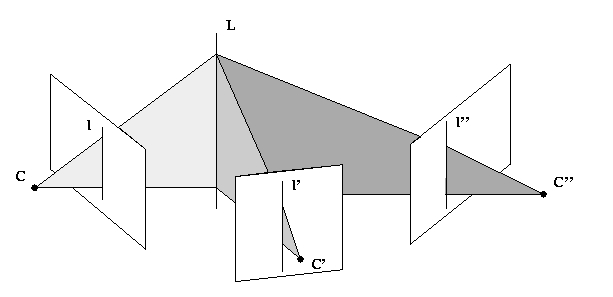
\includegraphics[width=100mm]{figures/threeviews.jpg}
  \caption{Trifocal geometry of three views}
  \label{fig:threeviews}
\end{figure}

Let $ l_i \leftrightarrow l^{\prime}_i \leftrightarrow l^{\prime \prime}_i $ be the set of corresponding lines of $L$. Let the camera matrices for the three views be $P =  \begin{bmatrix} I \mid 0 \end{bmatrix}$, $P^{\prime} = \begin{bmatrix} A \mid a_{4} \end{bmatrix}$, $P^{\prime \prime} = \begin{bmatrix} B \mid b_{4} \end{bmatrix}$, where $A$ and $B$ are $3 \times 3$ matrices, and the vectors $a_i$ and $b_i$ are the \texttt{i}-th columns of the respective camera matrices for $i = 1,\dotsb,4$. $A$ and $B$ are the homographies from the first to the second and third cameras respectively. Due to our choice for the first camera matrix, $a_4$ and $b_4$ are consequently the epipoles of the first camera in views two and three respectively.
 \begin{align*}
  a_4 &= e^{\prime} = P^{\prime}C  & b_4 &= e^{\prime \prime}  = P^{\prime \prime}C
 \end{align*}

Each image line back-projects to a plane as shown in Figure.\ref{fig:threeviews}. These planes are
\begin{align*}
\pi &= P^{T}l = \begin{pmatrix} l \\ 0 \end{pmatrix}  & \pi^{\prime} &= P^{\prime T}l^{\prime} = \begin{pmatrix} A^{T}l^{\prime} \\ a^{T}_{4}l^{\prime} \end{pmatrix} & \pi^{\prime \prime} &= P^{\prime \prime T}l^{\prime \prime} = \begin{pmatrix} B^{T}l^{\prime \prime} \\ b^{T}_{4}l^{\prime \prime} \end{pmatrix}
\end{align*}

The intersection constraint of the three planes in the common line in 3-space can be expressed algebraically by the requirement that the $4 \times 3$ matrix $ M = \begin{bmatrix} \pi & \pi^{\prime} & \pi^{\prime \prime} \end{bmatrix}$ has rank $2$. Points on the line of intersection may be represented as $X = \alpha X_1 + \beta X_2$, with $X_1$ and $X_2$ linearly independent. Such points lie on all three planes and so $\pi^{T}X = \pi^{\prime T}X = \pi^{\prime \prime T}X = 0$. It follows that $M^{T}X = 0$. Consequently M has a 2-dimensional null-space since $M^{T}X_1 = 0$ and $M^{T}X_2 =0$.

Since the rank of $M$ is 2, there is a linear dependence between its columns $m_i$, such that.
\begin{gather*}
M = \begin{bmatrix} m_1, m_2,m_3 \end{bmatrix} = \begin{bmatrix} l & A^{T}l^{\prime} & B^{T}l^{\prime \prime} \\
  0 & a^{T}_{4}l^{\prime} & b^{T}_{4}l^{\prime \prime}
\end{bmatrix}\\
m_1 = \alpha m_2 + \beta m_3
\end{gather*}

From the 2nd row of $M$, $\alpha = k(b^{T}_4 l^{\prime \prime})$ and $\beta = -k(a^{T}_4 l^{\prime})$ for some scalar $k$. Applying this back to the 1st row get
\begin{gather*}
l = (b^{T}_4 l^{\prime \prime })A^{T}l^{\prime} - (a^{T}_4 l^{\prime})B^{T}l^{\prime \prime}\\
l = (l^{\prime \prime T} b_{4})A^{T}l^{\prime} - (l^{\prime T} a_{4})B^{T}l^{\prime \prime}
\end{gather*}

The \texttt{i}-th coordinate $l_i$ of $l$ may be written as
\begin{gather*}
  l_i = l^{\prime \prime T} (b_{4}a^{T}_{i}) l^{\prime} - l^{\prime T}(a_{4}b^{T}_{i}) l^{\prime \prime}\\
  l_i = l^{\prime T} (a_{i}b^{T}_{4}) l^{\prime \prime} - l^{\prime T}(a_{4}b^{T}_{i}) l^{\prime \prime}
\end{gather*}

This relationship can be expressed with the permutation tensor such as
\begin{gather}
  \mathcal{T}_{i} = a_{i}b^{T}_{4} - a_{4}b^{T}_{i} \label{eq:trifocalgeometry1}\\
  l_i = l^{\prime T} \mathcal{T}_{i} l^{\prime \prime} \label{eq:trifocalgeometry2}
\end{gather}

$\mathcal{T}$ is then the trifocal tensor relating the 3 views together. It has 27 elements. There are 26 independent rations apart from the common overall scaling factor of the tensor. However, the tensor has only 18 independent degrees of freedom. Each of 3 camera matrices has 11 degrees of freedom which makes $33$ in total. However, $15$ degrees of freedom must be subtracted to account for the projective world frame, thus leaving 18 degrees of freedom.

\begin{figure}[ht!]
  \centering
  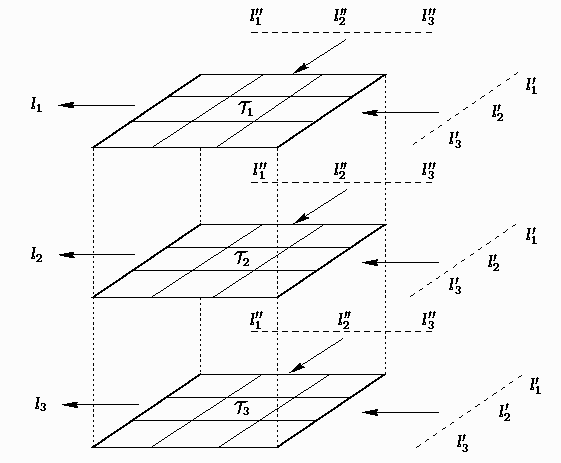
\includegraphics[width=100mm]{figures/trifocaltensor.png}
  \caption{A 3D representation of the trifocal tensor $l_{i} = l_{j}^{\prime} l_{k}^{\prime \prime} \mathcal{T}_{i}^{jk}$ }
  \label{fig:trifocaltensor}
\end{figure}

A point $x$ on the line $l$ must satisfy $x^{T}l = \sum_{i} x^{i}l_{i} = 0$. From \eqref{eq:trifocalgeometry2}, this may be written as
$
l^{\prime T}(\sum_{i} x^{i}\mathcal{T}_{i}) l^{\prime \prime} = 0
$
which means that there exists a 3D point $X$ mapping to $x$ in the first image, and to points on the lines $l^{\prime}$ and $l^{\prime \prime}$ in the second and third images. It's the incidence relationship that holds point-line-line correspondence.

To develop the point-point-point correspondence relationship, we can explore the homography map between the points on first and third images given by $x^{\prime \prime} = Hx$ and $l = H^{T}l^{\prime \prime}$. Thus we get
$$
  h_i = \mathcal{T}^{T}_{i}l^{\prime}
$$
Similarly, the homography from the first to the second views
$$
  h_i = \mathcal{T}_{i}l^{\prime \prime}
$$

Using these results back to our point-line-line correspondence relation,
\begin{gather*}
  x^{\prime \prime} = (\sum_{i} x^{i}\mathcal{T}^{T}_{i}) l^{\prime}
  x^{\prime \prime T}[x^{\prime \prime}]_{\times} = l^{\prime T} (\sum_{i} x^{i}\mathcal{T}_{i})[x^{\prime \prime}]_{\times} = 0^{T}
\end{gather*}

The line $l^{\prime}$ passes through $x^{\prime}$ may be written as $l^{\prime} = [x^{\prime}]_{\times}y^{\prime}$ for some point $y^{\prime}$ on $l^{\prime}$. Then
$$
  y^{\prime T} [x^{\prime}]_{times} (\sum_{i} x^{i}\mathcal{T}_{i})[x^{\prime \prime}]_{\times} = 0^{T}
$$

This relation holds true for all lines $l^{\prime}$ through $x^{\prime}$ and so is independent of $y^{\prime}$, hence this relation can be written as
$$
[x^{\prime}]_{times} (\sum_{i} x^{i}\mathcal{T}_{i})[x^{\prime \prime}]_{\times} = 0_{3\times 3}
$$
which expresses the point-point-point coincidence relationship required. Expressing this relation in proper tensor notation is then given by
\begin{equation}
  x^{i}(x^{\prime j} \epsilon_{jpr})(x^{\prime \prime k} \epsilon_{kqs})\mathcal{T}^{pq}_{i} = 0_{rs} \label{eq:trifocalgeometry3}
\end{equation}

\subsection{Recovering Projection Matrices}
\label{sub:recovering_projection_matrices}
Since the trifocal tensor embeds the geometry of the three cameras in our scene, this implies that the camera matrices may be computed from the trifocal tensor up to a projective ambiguity~\cite{Hartley2004}.

First, the epipoles $e^{\prime},e^{\prime \prime}$ are retrieved. Let $u_i$ and $v_i$ be the left and right null-vectors respectively of $\mathcal{T}_{i}$, \textit{i.e.:} $u_{i}^{T} \mathcal{T}_{i} = {\bf 0}^{T}, \mathcal{T}_{i}v_i = 0$. Then the epipoles are obtained as the null vectors to the following $ 3 \times 3$ matrices:
\begin{equation}
  e^{\prime T} [u_1, u_2, u_3] = 0  \text{ and } e^{\prime \prime T}[v_1, v_2, v_3] = 0
  \label{eq:recoveringepipoles}
\end{equation}

Next, to retrieve the camera matrices $P^{\prime}, P^{\prime \prime}$. The epipoles are normalized to unit norm, then:
\begin{equation}
  P^{\prime} = [[\mathcal{T}_{1}, \mathcal{T}_{2},\mathcal{T}_{3}] e^{\prime \prime} | e^{\prime}] \text{ and } P^{\prime \prime} = [(e^{\prime \prime} e^{\prime \prime T} - I)[\mathcal{T}_{1}^{T}, \mathcal{T}_{2}^{T},\mathcal{T}_{3}^{T}] e^{\prime} | e^{\prime \prime}]
\end{equation}

\subsection{Estimating Trifocal Tensor}
The trifocal tensor can be computed from feature correspondences across the three views. Computation of tensor using correspondences of points or lines has been studied extensively in literature. The main linear algorithm presented by \texttt{Hartley}\cite{Hartley2004} is the straightforward method to compute the tensor. Other methods make use of \texttt{RANSAC} (RANdom SAmple Consensus) to enable the tensor estimation to be robust to outliers that usually cause the linear algebraic method to fail \cite{torr1997robust}.

Each triplet of corresponding image points gives 4 equations linearly independent. Therefore, a minimum set of 7 correspondences of points are needed for the trifocal tensor computation to uniquely determine the 27 entries of the tensor matrix. Given $n$ point correspondences, let $A$ be a matrix of size $4n \times 27$ and $t$ a vector containing all entires of the tensor, then we have
\begin{equation}
  At = 0
  \label{eq:tensorsvd}
\end{equation}
By applying the least square method or SVD, the tensor is obtained from the solution to this linear system. However, \texttt{Hartley} has shown that this kind of algorithm does not do well if all the points are of the form $(x_1, x_2, 1)$ in homogeneous coordinates with $x_1$ and $x_2$ very much larger than $1$. Therefore, it is necessary to normalize the points of each image separately before computing the tensor. The points are translated in each image so that the centroid of all measured points is at the origin of the image coordinates, and then scaled so that the average distance of a point from the origin is $\sqrt{2}$ units. This way the average point will be something like $(1, 1 ,1)$ in homogeneous coordinates, and each of the homogeneous coordinate will be approximately of equal weight. This transformation improves the condition of the matrix of equations and leads to a better solution. Consequently, a de-normalization step is needed in order to work with the original image coordinates.

This method still suffers from two issues
\begin{enumerate}
  \item The tensor is parameterized by all its entries and this does not take into account the tensor geometrical constraints. Therefore, there is always a risk of obtaining an invalid tensor.
  \item Using all available point correspondences causes the tensor to be significantly affected by the presence of strong outliers.
\end{enumerate}

Hence, an algebraic minimization is needed there after, to use the linear solution as an initial estimate and re-parameterize it by the 24 entries of the projection matrices $P^\prime$ and $P^{\prime \prime}$. The desired tensor is found by minimizing the residual error. The overall procedure is briefly explained here.
\begin{enumerate}
  \item Normalize the set of point triplets by performing transformations $H$, $H^{\prime}$ and $H^{\prime \prime}$. Here $\hat{x} = Hx$, $\hat{x}^{\prime} = H^{\prime}x^{\prime}$, $\hat{x}^{\prime \prime} = H^{\prime \prime} x^{\prime \prime}$.
  \item Compute the tensor linearly by solving a set of equations of the form $At = 0$, where $A$ expresses~\ref{eq:trifocalgeometry3}, and $t$ is the vector of entries of the tensor.
  \item De-normalize the tensor by $T_i = H^{\prime -1} \sum_{j}(H^{T}(i,j)T_j)H^{\prime \prime -T}$
  \item Find the two epipoles $e^{\prime}$ and $e^{\prime \prime}$ from the tensor using~\ref{eq:recoveringepipoles}.
  \item According to Equation~\ref{eq:trifocalgeometry1}, construct the $28 \times 12$ matrix $E$ such that $t = Ea$, where $a$ is the vector representing entries of $a_i$ and $b_i$.
  \item Compute the tensor by minimizing the algebraic error $AEa$ subject to $Ea = 1$.
\end{enumerate}

The above algorithm leads to a geometrically valid tensor because its entries satisfies the equation~\ref{eq:trifocalgeometry1}. However, the main weakness of the algebraic minimization method is that all point correspondences are involved in the tensor computation and still suffers from outliers in practice.



\section{Visual Servoing}


\section{Previous Works}

\chapter{Methodology} \label{chap:methodology}

In this chapter, we present the development of a visual servoing method based on using the trifocal tensor elements as visual features in our visual servoing control loop. We begin by developing the needed control law using the tensor, finding the respective interaction matrix, and then exploring the normalization approach for the obtained tensor and interaction matrix. Finally we represent the overall procedure for the proposed algorithm to be implemented.

\section{Control Law}
To formulate the control law of the trifocal tensor based visual servoing, we need to establish the model of the system and find the relation between the input of the control and the trifocal tensor coefficients. The trifocal tensor can be computed from feature correspondences across the three views. Our goal is to find the interaction matrix relating the control input and the tensor derivatives.
\begin{equation}
  \dot{\mathcal{T}}_{(jkl)} = L_{\mathcal{T}_{(jkl)}} \begin{pmatrix} v_c \\ w_c \end{pmatrix}
\end{equation}

\subsection{Coefficients of the Trifocal Tensor}
To compute the relation between the coefficients of the trifocal tensor and the Projective matrices, first we write the Tensor relation \eqref{eq:trifocalgeometry1} with the proper visual servoing notation as follows
\begin{equation}
  \mathcal{T}_{(jkl)} = a_{(kj)}b_{(4l)} - a_{(4k)}b_{(lj)} \label{eq:tensorrelation}
\end{equation}

For the sake of maintaining the Visual Servoing convention, we omit the use of $i$ as an index for the tensor relation. The letter $i$ further on will be indicating the initial view in the control system. The Camera positions are then written as $C_{c^*},C_c,C_i$ for the desired, current, and initial camera positions respectively. The same may also be done for the projection matrices, and instead of using the matrices $A,B$ to express the homography between the first and second or third views, we will use the standard notation from Visual Servoing with the corresponding Rotation matrices $^{c}R_{c^*}, ^{i}R_{c^*}$ respectively. For the translations $a_4, b_4$, we will use $^{c}{t}_{c^*}, ^{i}{t}_{c^*}$ respectively. Leading superscripts will denote the frame with respect to which a set of coordinates are defined. Thus, the rotation matrix $^{c}R_{c^*}$ gives the orientation of the desired camera frame relative to the current camera frame.

\begin{align*}
  C &\Rightarrow C_{c^*} \text{  Desired camera position} \\
  C' &\Rightarrow C_c \text{  Current camera position} \\
  C^{''} &\Rightarrow C_i \text{  Initial camera position} \\
\end{align*}
\begin{gather*}
  P_d = P = [I | 0]\\
  P_c = P^{\prime} = [A | a_4] : ^{c}{\bf M}_{c^*} = [ ^{c}{\bf R}_{c^*} | ^{c}{\bf t}_{c^*} ]\\
  P_i = P^{\prime \prime} = [B | b_4] : ^{i}{\bf M}_{c^*} = [ ^{i}{\bf R}_{c^*} | ^{i}{\bf t}_{c^*} ]
\end{gather*}

The Tensor relation \eqref{eq:tensorrelation} can then be expressed as follows
\begin{equation}
\mathcal{T}_{(jkl)} = \tensor[^{c}]{R}{_{c^{*}(kj)}} \ \tensor[^{i}]{t}{_{c^{*}(l)}} - \tensor[^{c}]{t}{_{c^{*}(k)}} \ \tensor[^{i}]{R}{_{c^{*}(lj)}} \label{eq:tensorcoeffs}
\end{equation}

Expanding this relation further to compute the tensor coefficients is straight forward, expanding for values of $j,k,l$ we get the following tensor coefficients:

\begin{equation}
\begin{gathered}
  \mathcal{T}_{(111)} = \tensor[^{c}]{R}{_{c^{*}(11)}} \ \tensor[^{i}]{t}{_{c^{*}(1)}} - \tensor[^{c}]{t}{_{c^{*}(1)}} \ \tensor[^{i}]{R}{_{c^{*}(11)}}\\
  \mathcal{T}_{(112)} = \tensor[^{c}]{R}{_{c^{*}(11)}} \ \tensor[^{i}]{t}{_{c^{*}(2)}} - \tensor[^{c}]{t}{_{c^{*}(1)}} \ \tensor[^{i}]{R}{_{c^{*}(21)}}\\
  \mathcal{T}_{(113)} = \tensor[^{c}]{R}{_{c^{*}(11)}} \ \tensor[^{i}]{t}{_{c^{*}(3)}} - \tensor[^{c}]{t}{_{c^{*}(1)}} \ \tensor[^{i}]{R}{_{c^{*}(31)}}\\
  \mathcal{T}_{(121)} = \tensor[^{c}]{R}{_{c^{*}(21)}} \ \tensor[^{i}]{t}{_{c^{*}(1)}} - \tensor[^{c}]{t}{_{c^{*}(2)}} \ \tensor[^{i}]{R}{_{c^{*}(11)}}\\
  \mathcal{T}_{(122)} = \tensor[^{c}]{R}{_{c^{*}(21)}} \ \tensor[^{i}]{t}{_{c^{*}(2)}} - \tensor[^{c}]{t}{_{c^{*}(2)}} \ \tensor[^{i}]{R}{_{c^{*}(21)}}\\
  \mathcal{T}_{(123)} = \tensor[^{c}]{R}{_{c^{*}(21)}} \ \tensor[^{i}]{t}{_{c^{*}(3)}} - \tensor[^{c}]{t}{_{c^{*}(2)}} \ \tensor[^{i}]{R}{_{c^{*}(31)}}\\
  \mathcal{T}_{(131)} = \tensor[^{c}]{R}{_{c^{*}(31)}} \ \tensor[^{i}]{t}{_{c^{*}(1)}} - \tensor[^{c}]{t}{_{c^{*}(3)}} \ \tensor[^{i}]{R}{_{c^{*}(11)}}\\
  \mathcal{T}_{(132)} = \tensor[^{c}]{R}{_{c^{*}(31)}} \ \tensor[^{i}]{t}{_{c^{*}(2)}} - \tensor[^{c}]{t}{_{c^{*}(3)}} \ \tensor[^{i}]{R}{_{c^{*}(21)}}\\
  \mathcal{T}_{(133)} = \tensor[^{c}]{R}{_{c^{*}(31)}} \ \tensor[^{i}]{t}{_{c^{*}(3)}} - \tensor[^{c}]{t}{_{c^{*}(3)}} \ \tensor[^{i}]{R}{_{c^{*}(31)}}\\
  \mathcal{T}_{(211)} = \tensor[^{c}]{R}{_{c^{*}(12)}} \ \tensor[^{i}]{t}{_{c^{*}(1)}} - \tensor[^{c}]{t}{_{c^{*}(1)}} \ \tensor[^{i}]{R}{_{c^{*}(12)}}\\
  \mathcal{T}_{(212)} = \tensor[^{c}]{R}{_{c^{*}(12)}} \ \tensor[^{i}]{t}{_{c^{*}(2)}} - \tensor[^{c}]{t}{_{c^{*}(1)}} \ \tensor[^{i}]{R}{_{c^{*}(22)}}\\
  \mathcal{T}_{(213)} = \tensor[^{c}]{R}{_{c^{*}(12)}} \ \tensor[^{i}]{t}{_{c^{*}(3)}} - \tensor[^{c}]{t}{_{c^{*}(1)}} \ \tensor[^{i}]{R}{_{c^{*}(32)}}\\
  \mathcal{T}_{(221)} = \tensor[^{c}]{R}{_{c^{*}(22)}} \ \tensor[^{i}]{t}{_{c^{*}(1)}} - \tensor[^{c}]{t}{_{c^{*}(2)}} \ \tensor[^{i}]{R}{_{c^{*}(12)}}\\
  \mathcal{T}_{(222)} = \tensor[^{c}]{R}{_{c^{*}(22)}} \ \tensor[^{i}]{t}{_{c^{*}(2)}} - \tensor[^{c}]{t}{_{c^{*}(2)}} \ \tensor[^{i}]{R}{_{c^{*}(22)}}\\
  \mathcal{T}_{(223)} = \tensor[^{c}]{R}{_{c^{*}(22)}} \ \tensor[^{i}]{t}{_{c^{*}(3)}} - \tensor[^{c}]{t}{_{c^{*}(2)}} \ \tensor[^{i}]{R}{_{c^{*}(32)}}\\
  \mathcal{T}_{(231)} = \tensor[^{c}]{R}{_{c^{*}(32)}} \ \tensor[^{i}]{t}{_{c^{*}(1)}} - \tensor[^{c}]{t}{_{c^{*}(3)}} \ \tensor[^{i}]{R}{_{c^{*}(12)}}\\
  \mathcal{T}_{(232)} = \tensor[^{c}]{R}{_{c^{*}(32)}} \ \tensor[^{i}]{t}{_{c^{*}(2)}} - \tensor[^{c}]{t}{_{c^{*}(3)}} \ \tensor[^{i}]{R}{_{c^{*}(22)}}\\
  \mathcal{T}_{(233)} = \tensor[^{c}]{R}{_{c^{*}(32)}} \ \tensor[^{i}]{t}{_{c^{*}(3)}} - \tensor[^{c}]{t}{_{c^{*}(3)}} \ \tensor[^{i}]{R}{_{c^{*}(32)}}\\
  \mathcal{T}_{(311)} = \tensor[^{c}]{R}{_{c^{*}(13)}} \ \tensor[^{i}]{t}{_{c^{*}(1)}} - \tensor[^{c}]{t}{_{c^{*}(1)}} \ \tensor[^{i}]{R}{_{c^{*}(13)}}\\
  \mathcal{T}_{(312)} = \tensor[^{c}]{R}{_{c^{*}(13)}} \ \tensor[^{i}]{t}{_{c^{*}(2)}} - \tensor[^{c}]{t}{_{c^{*}(1)}} \ \tensor[^{i}]{R}{_{c^{*}(23)}}\\
  \mathcal{T}_{(313)} = \tensor[^{c}]{R}{_{c^{*}(13)}} \ \tensor[^{i}]{t}{_{c^{*}(3)}} - \tensor[^{c}]{t}{_{c^{*}(1)}} \ \tensor[^{i}]{R}{_{c^{*}(33)}}\\
  \mathcal{T}_{(321)} = \tensor[^{c}]{R}{_{c^{*}(23)}} \ \tensor[^{i}]{t}{_{c^{*}(1)}} - \tensor[^{c}]{t}{_{c^{*}(2)}} \ \tensor[^{i}]{R}{_{c^{*}(13)}}\\
  \mathcal{T}_{(322)} = \tensor[^{c}]{R}{_{c^{*}(23)}} \ \tensor[^{i}]{t}{_{c^{*}(2)}} - \tensor[^{c}]{t}{_{c^{*}(2)}} \ \tensor[^{i}]{R}{_{c^{*}(23)}}\\
  \mathcal{T}_{(323)} = \tensor[^{c}]{R}{_{c^{*}(23)}} \ \tensor[^{i}]{t}{_{c^{*}(3)}} - \tensor[^{c}]{t}{_{c^{*}(2)}} \ \tensor[^{i}]{R}{_{c^{*}(33)}}\\
  \mathcal{T}_{(331)} = \tensor[^{c}]{R}{_{c^{*}(33)}} \ \tensor[^{i}]{t}{_{c^{*}(1)}} - \tensor[^{c}]{t}{_{c^{*}(3)}} \ \tensor[^{i}]{R}{_{c^{*}(13)}}\\
  \mathcal{T}_{(332)} = \tensor[^{c}]{R}{_{c^{*}(33)}} \ \tensor[^{i}]{t}{_{c^{*}(2)}} - \tensor[^{c}]{t}{_{c^{*}(3)}} \ \tensor[^{i}]{R}{_{c^{*}(23)}}\\
  \mathcal{T}_{(333)} = \tensor[^{c}]{R}{_{c^{*}(33)}} \ \tensor[^{i}]{t}{_{c^{*}(3)}} - \tensor[^{c}]{t}{_{c^{*}(3)}} \ \tensor[^{i}]{R}{_{c^{*}(33)}}
\end{gathered}\label{eq:tensorcoeffsexpanded}
\end{equation}

\pagebreak

Our objective is to move our robot from the initial camera position to the desired target camera position. Therefore, we have two special cases for the tensor coefficients values.
\begin{description}
  \item[First when $C_c$ at the initial position $C_i$] \hfill
    \begin{equation}
    \begin{gathered}
      \tensor[^{c}]{R}{_{c^{*}}} = \tensor[^{i}]{R}{_{c^{*}}}, \ \tensor[^{c}]{t}{_{c^{*}}} = \tensor[^{i}]{t}{_{c^{*}}}\\
      \mathcal{T}_{(jkl)}^{i} = \tensor[^{c}]{R}{_{c^{*}(kj)}} \ \tensor[^{c}]{t}{_{c^{*}(l)}} - \tensor[^{c}]{t}{_{c^{*}(k)}} \ \tensor[^{c}]{R}{_{c^{*}(lj)}}\\
      \text{when } k = l, \mathcal{T}_{(jkl)}^{i} = 0\\
      \mathcal{T}_{(112)}^{i} = -\mathcal{T}_{(121)}^{i}, \mathcal{T}_{(113)}^{i} = -\mathcal{T}_{(131)}^{i}, \mathcal{T}_{(123)}^{i} = -\mathcal{T}_{(132)}^{i}\\
      \mathcal{T}_{(212)}^{i} = -\mathcal{T}_{(221)}^{i}, \mathcal{T}_{(213)}^{i} = -\mathcal{T}_{(231)}^{i}, \mathcal{T}_{(223)}^{i} = -\mathcal{T}_{(232)}^{i}\\
      \mathcal{T}_{(312)}^{i} = -\mathcal{T}_{(321)}^{i}, \mathcal{T}_{(313)}^{i} = -\mathcal{T}_{(331)}^{i}, \mathcal{T}_{(323)}^{i} = -\mathcal{T}_{(332)}^{i}
    \end{gathered}\label{eq:tensorcoeffinitial}
    \end{equation}
  \item[Second when $C_c$ at the desired position $C_{c^*}$] \hfill
    \begin{equation}
    \begin{gathered}
      \tensor[^{c}]{R}{_{c^{*}}} = I, \ \tensor[^{c}]{t}{_{c^{*}}} = \bf{0}\\
      \mathcal{T}_{(jkl)}^{*} = I_{(kj)} \ \tensor[^{i}]{t}{_{c^{*}(l)}}\\
      \text{when } j \neq k, \mathcal{T}_{(jkl)}^{*} = 0\\
      \mathcal{T}_{(111)}^{*} = \mathcal{T}_{(221)}^{*} = \mathcal{T}_{(331)}^{*} = \tensor[^{i}]{t}{_{c^{*}(1)}}\\
      \mathcal{T}_{(112)}^{*} = \mathcal{T}_{(222)}^{*} = \mathcal{T}_{(332)}^{*} = \tensor[^{i}]{t}{_{c^{*}(2)}}\\
      \mathcal{T}_{(113)}^{*} = \mathcal{T}_{(223)}^{*} = \mathcal{T}_{(333)}^{*} = \tensor[^{i}]{t}{_{c^{*}(3)}}
    \end{gathered}\label{eq:tensorcoeffdesired}
  \end{equation}
\end{description}

\subsection{Tensor Derivation}
\label{sub:tensor_derivation}

First, The derivatives of all the trifocal tensor elements with respect to time are generally as following:
\begin{equation}
  \dot{\mathcal{T}}_{(jkl)} = \tensor[^{c}]{\dot{R}}{_{c^{*}(kj)}} \ \tensor[^{i}]{t}{_{c^{*}(l)}} + \tensor[^{c}]{R}{_{c^{*}(kj)}} \ \tensor[^{i}]{\dot{t}}{_{c^{*}(l)}} - \tensor[^{c}]{\dot{t}}{_{c^{*}(k)}} \ \tensor[^{i}]{R}{_{c^{*}(lj)}} - \tensor[^{c}]{t}{_{c^{*}(k)}} \ \tensor[^{i}]{\dot{R}}{_{c^{*}(lj)}} \label{eq:tensorderivatives1}
\end{equation}

Since our initial camera $C_i$ is fixed, the elements of the derivatives of its rotation matrix and its transpose vector are equal to zero, \textit{i.e.:} $\tensor[^i]{\dot{t}}{_{c^{*}(l)}} = \tensor[^i]{\dot{R}}{_{c^{*}(jl)}} = 0$. Our trifocal tensor elements derivative is then simplified to:
\begin{equation}
  \dot{\mathcal{T}}_{(jkl)} = \tensor[^{c}]{\dot{R}}{_{c^{*}(kj)}} \ \tensor[^{i}]{t}{_{c^{*}(l)}} - \tensor[^{c}]{\dot{t}}{_{c^{*}(k)}} \ \tensor[^{i}]{R}{_{c^{*}(lj)}} \label{eq:tensorderivatives2}
\end{equation}

The spatial velocity of the camera is $u_c = {(v_c, \omega_{c})}^{T}$, where $v_c$ and $\omega_c$ are the translational and rotational velocities of the camera. From the geometry of the scene, we can deduce the following relationships:
\begin{gather*}
  {[\omega_{c}]}_{\times} = \tensor[^{c^*}]{R}{_{c}^{T}} \tensor[^{c^*}]{\dot{R}}{_{c}} = - \tensor[^{c^*}]{\dot{R}}{_{c}^{T}} \tensor[^{c^*}]{R}{_{c}}\\
  \tensor[^{c^*}]{\dot{R}}{_{c}^{T}} = - {[\omega_{c}]}_{\times}\tensor[^{c^*}]{R}{_{c}^{T}}\\
  \tensor[^{c^*}]{\dot{R}}{_{c}^{T}} = - {[\omega_{c}]}_{\times}\tensor[^{c}]{R}{_{c^*}}\\
  \tensor[^{c}]{\dot{R}}{_{c^*}} = -{[\omega_c]}_{\times}\tensor[^{c}]{R}{_{c^*}}\\
  %
  \tensor[^{c^*}]{\dot{t}}{_{c}} = \tensor[^{c^*}]{R}{_{c}}v_{c}\\
  \tensor[^{c}]{t}{_{c^*}} = - \tensor[^{c}]{R}{_{c^*}} \tensor[^{c^*}]{t}{_{c}}\\
  \tensor[^{c}]{\dot{t}}{_{c^*}} = - \tensor[^{c}]{\dot{R}}{_{c^*}} \tensor[^{c^*}]{t}{_{c}} - \tensor[^{c}]{R}{_{c^*}} \tensor[^{c^*}]{\dot{t}}{_{c}}\\
  \tensor[^{c}]{\dot{t}}{_{c^*}} = {[\omega_c]}_{\times}\tensor[^{c}]{R}{_{c^*}} \tensor[^{c^*}]{t}{_{c}} - \tensor[^{c}]{R}{_{c^*}} \tensor[^{c^*}]{R}{_{c}}v_{c}\\
  \tensor[^{c}]{\dot{t}}{_{c^*}} = {[\omega_c]}_{\times}\tensor[^{c}]{t}{_{c^*}} - v_{c}\\
  \tensor[^{c}]{\dot{t}}{_{c^*}} = {[\tensor[^{c}]{t}{_{c^*}}]}_{\times}\omega_c - v_{c}\\
%
  \tensor[^{c}]{\dot{t}}{_{c^{*}(k)}} = [-I | {[\tensor[^{c}]{t}{_{c^*}}]}_{\times}] u
\end{gather*}

Substituting back into the tensor derivation \eqref{eq:tensorderivatives2}, we get:
\begin{equation}
\begin{gathered}
  \dot{\mathcal{T}}_{(jkl)} =  - {({[\omega_c]}_{\times}\tensor[^{c}]{R}{_{c^*}})}_{(kj)}\ \tensor[^{i}]{t}{_{c^*(l)}} - {({[\tensor[^{c}]{t}{_{c^*}}]}_{\times}\omega_c - v_{c})}_{(k)}\ \tensor[^{i}]{R}{_{c^*(lj)}}\\
  \dot{\mathcal{T}}_{(jkl)} =  - (\sum_{m}{[\omega_{c}]}_{\times(km)}\tensor[^{c}]{R}{_{c^*(mj)}})\ \tensor[^{i}]{t}{_{c^*(l)}} - ({({[\tensor[^{c}]{t}{_{c^*}}]}_{\times}\omega_c)}_{(k)}  -   v_{c(k)})\ \tensor[^{i}]{R}{_{c^*(lj)}}
\end{gathered}\label{eq:tensorderivatives3}
\end{equation}

where
\begin{gather*}
\tensor[^{i}]{t}{_{c^*}} = -\tensor[^{i}]{R}{_{c^*}}\begin{pmatrix} x_i \\ y_i \\ z_i \end{pmatrix}, \
\tensor[^{c}]{t}{_{c^*}} = -\tensor[^{c}]{R}{_{c^*}}\begin{pmatrix} x_c \\ y_c \\ z_c \end{pmatrix}, \\
  \tensor[^{i}]{R}{_{c^*}} = \begin{bmatrix}
    R_{i(11)} & R_{i(12)} & R_{i(13)} \\
    R_{i(21)} & R_{i(22)} & R_{i(23)} \\
    R_{i(31)} & R_{i(32)} & R_{i(33)}
  \end{bmatrix},\
\tensor[^{c}]{R}{_{c^*}} = \begin{bmatrix}
  R_{c(11)} & R_{c(12)} & R_{c(13)} \\
  R_{c(21)} & R_{c(22)} & R_{c(23)} \\
  R_{c(31)} & R_{c(32)} & R_{c(33)}
\end{bmatrix},\\
{[\omega_{c}]}_{\times} = \begin{bmatrix} 0 & -\omega_z & \omega_y \\ \omega_z & 0 & -\omega_y \\ -\omega_y & \omega_x & 0 \end{bmatrix},\
{[\tensor[^{c}]{t}{_{c^*}}]}_{\times}\omega_c  = \begin{bmatrix} -\tensor[^{c}]{t}{_{c^*(3)}}\omega_y + \tensor[^{c}]{t}{_{c^*(2)}} \omega_z \\\ \ \tensor[^{c}]{t}{_{c^*(3)}}\omega_x - \tensor[^{c}]{t}{_{c^*(1)}} \omega_z \\ -\tensor[^{c}]{t}{_{c^*(2)}}\omega_x + \tensor[^{c}]{t}{_{c^*(1)}}\omega_y \end{bmatrix}
\end{gather*}

From~\eqref{eq:tensorcoeffsexpanded} and~\eqref{eq:tensorderivatives3}, the derivative of the first tensor coefficient can be computed as follows:
\begin{equation}
\begin{gathered}
  \dot{\mathcal{T}}_{(111)} =  - (-R_{c(21)} \omega_z + R_{c(31)}\omega_y)\ \tensor[^{i}]{t}{_{c^*(1)}} - (-\tensor[^{c}]{t}{_{c^*(3)}}\omega_y + \tensor[^{c}]{t}{_{c^*(2)}} \omega_z - v_x)\ \tensor[^{i}]{R}{_{c^*(11)}}\\
  \dot{\mathcal{T}}_{(111)} = R_{i(11)}v_x - (R_{c(31)}\tensor[^{i}]{t}{_{c^*(1)}} - R_{i(11)}\tensor[^{c}]{t}{_{c^*(3)}}) \omega_y  + (R_{c(21)}\tensor[^{i}]{t}{_{c^*(1)}} - R_{i(11)}\tensor[^{c}]{t}{_{c^*(2)}} ) \omega_z\\
  \dot{\mathcal{T}}_{(111)} = R_{i(11)}v_x - \mathcal{T}_{(131)} \omega_y  +  \mathcal{T}_{(121)} \omega_z
\end{gathered}
\end{equation}

By expanding the derivatives for the rest of the coefficients, we can deduce this compact form for the tensor coefficients derivatives:
\begin{equation}
\begin{gathered}
  \dot{\mathcal{T}}_{(jkl)} = R_{i(lj)}v_{c(k)} - \sum_{m} {[\omega_{c}]}_{\times(km)} \mathcal{T}_{(jml)}
%%  \dot{\mathcal{T}}_{(111)} =  - (-R_{c(21)} \omega_z + R_{c(31)}\omega_y)\ \tensor[^{i}]{t}{_{c^*(1)}} - (-\tensor[^{c}]{t}{_{c^*(3)}}\omega_y + \tensor[^{c}]{t}{_{c^*(2)}} \omega_z -v_x)\ \tensor[^{i}]{R}{_{c^*(11)}}\\
%%  \dot{\mathcal{T}}_{(112)} =  - (-R_{c(21)} \omega_z + R_{c(31)}\omega_y)\ \tensor[^{i}]{t}{_{c^*(2)}} - (-\tensor[^{c}]{t}{_{c^*(3)}}\omega_y + \tensor[^{c}]{t}{_{c^*(2)}} \omega_z -v_x)\ \tensor[^{i}]{R}{_{c^*(21)}}\\
%%  \dot{\mathcal{T}}_{(113)} =  - (-R_{c(21)} \omega_z + R_{c(31)}\omega_y)\ \tensor[^{i}]{t}{_{c^*(3)}} - (-\tensor[^{c}]{t}{_{c^*(3)}}\omega_y + \tensor[^{c}]{t}{_{c^*(2)}} \omega_z -v_x)\ \tensor[^{i}]{R}{_{c^*(31)}}\\
%%  %
%%  \dot{\mathcal{T}}_{(121)} =  - ( R_{c(11)} \omega_z - R_{c(31)}\omega_x)\ \tensor[^{i}]{t}{_{c^*(1)}} - ( \tensor[^{c}]{t}{_{c^*(3)}}\omega_x - \tensor[^{c}]{t}{_{c^*(1)}} \omega_z -v_y)\ \tensor[^{i}]{R}{_{c^*(11)}}\\
%%  \dot{\mathcal{T}}_{(122)} =  - ( R_{c(11)} \omega_z - R_{c(31)}\omega_x)\ \tensor[^{i}]{t}{_{c^*(2)}} - ( \tensor[^{c}]{t}{_{c^*(3)}}\omega_x - \tensor[^{c}]{t}{_{c^*(1)}} \omega_z -v_y)\ \tensor[^{i}]{R}{_{c^*(21)}}\\
%%  \dot{\mathcal{T}}_{(123)} =  - ( R_{c(11)} \omega_z - R_{c(w1)}\omega_x)\ \tensor[^{i}]{t}{_{c^*(3)}} - ( \tensor[^{c}]{t}{_{c^*(3)}}\omega_x - \tensor[^{c}]{t}{_{c^*(1)}} \omega_z -v_y)\ \tensor[^{i}]{R}{_{c^*(31)}}\\
%%  %
%%  \dot{\mathcal{T}}_{(131)} =  - (-R_{c(11)} \omega_y + R_{c(21)}\omega_x)\ \tensor[^{i}]{t}{_{c^*(1)}} - (-\tensor[^{c}]{t}{_{c^*(2)}}\omega_x + \tensor[^{c}]{t}{_{c^*(1)}} \omega_y -v_z)\ \tensor[^{i}]{R}{_{c^*(11)}}\\
%%  \dot{\mathcal{T}}_{(132)} =  - (-R_{c(11)} \omega_y + R_{c(21)}\omega_x)\ \tensor[^{i}]{t}{_{c^*(2)}} - (-\tensor[^{c}]{t}{_{c^*(2)}}\omega_x + \tensor[^{c}]{t}{_{c^*(1)}} \omega_y -v_z)\ \tensor[^{i}]{R}{_{c^*(21)}}\\
%%  \dot{\mathcal{T}}_{(133)} =  - (-R_{c(11)} \omega_y + R_{c(21)}\omega_x)\ \tensor[^{i}]{t}{_{c^*(3)}} - (-\tensor[^{c}]{t}{_{c^*(2)}}\omega_x + \tensor[^{c}]{t}{_{c^*(1)}} \omega_y -v_z)\ \tensor[^{i}]{R}{_{c^*(31)}}\\
%%  %
%%  %
%%  \dot{\mathcal{T}}_{(211)} =  - (-R_{c(22)} \omega_z + R_{c(32)}\omega_y)\ \tensor[^{i}]{t}{_{c^*(1)}} - (-\tensor[^{c}]{t}{_{c^*(3)}}\omega_y + \tensor[^{c}]{t}{_{c^*(2)}} \omega_z -v_x)\ \tensor[^{i}]{R}{_{c^*(12)}}\\
%%  \dot{\mathcal{T}}_{(212)} =  - (-R_{c(22)} \omega_z + R_{c(32)}\omega_y)\ \tensor[^{i}]{t}{_{c^*(2)}} - (-\tensor[^{c}]{t}{_{c^*(3)}}\omega_y + \tensor[^{c}]{t}{_{c^*(2)}} \omega_z -v_x)\ \tensor[^{i}]{R}{_{c^*(22)}}\\
%%  \dot{\mathcal{T}}_{(213)} =  - (-R_{c(22)} \omega_z + R_{c(32)}\omega_y)\ \tensor[^{i}]{t}{_{c^*(3)}} - (-\tensor[^{c}]{t}{_{c^*(3)}}\omega_y + \tensor[^{c}]{t}{_{c^*(2)}} \omega_z -v_x)\ \tensor[^{i}]{R}{_{c^*(32)}}\\
%%  %
%%  \dot{\mathcal{T}}_{(221)} =  - ( R_{c(12)} \omega_z - R_{c(32)}\omega_x)\ \tensor[^{i}]{t}{_{c^*(1)}} - ( \tensor[^{c}]{t}{_{c^*(3)}}\omega_x - \tensor[^{c}]{t}{_{c^*(1)}} \omega_z -v_y)\ \tensor[^{i}]{R}{_{c^*(12)}}\\
%%  \dot{\mathcal{T}}_{(222)} =  - ( R_{c(12)} \omega_z - R_{c(32)}\omega_x)\ \tensor[^{i}]{t}{_{c^*(2)}} - ( \tensor[^{c}]{t}{_{c^*(3)}}\omega_x - \tensor[^{c}]{t}{_{c^*(1)}} \omega_z -v_y)\ \tensor[^{i}]{R}{_{c^*(22)}}\\
%%  \dot{\mathcal{T}}_{(223)} =  - ( R_{c(12)} \omega_z - R_{c(w2)}\omega_x)\ \tensor[^{i}]{t}{_{c^*(3)}} - ( \tensor[^{c}]{t}{_{c^*(3)}}\omega_x - \tensor[^{c}]{t}{_{c^*(1)}} \omega_z -v_y)\ \tensor[^{i}]{R}{_{c^*(32)}}\\
%%  %
%%  \dot{\mathcal{T}}_{(231)} =  - (-R_{c(12)} \omega_y + R_{c(22)}\omega_x)\ \tensor[^{i}]{t}{_{c^*(1)}} - (-\tensor[^{c}]{t}{_{c^*(2)}}\omega_x + \tensor[^{c}]{t}{_{c^*(1)}} \omega_y -v_z)\ \tensor[^{i}]{R}{_{c^*(12)}}\\
%%  \dot{\mathcal{T}}_{(232)} =  - (-R_{c(12)} \omega_y + R_{c(22)}\omega_x)\ \tensor[^{i}]{t}{_{c^*(2)}} - (-\tensor[^{c}]{t}{_{c^*(2)}}\omega_x + \tensor[^{c}]{t}{_{c^*(1)}} \omega_y -v_z)\ \tensor[^{i}]{R}{_{c^*(22)}}\\
%%  \dot{\mathcal{T}}_{(233)} =  - (-R_{c(12)} \omega_y + R_{c(22)}\omega_x)\ \tensor[^{i}]{t}{_{c^*(3)}} - (-\tensor[^{c}]{t}{_{c^*(2)}}\omega_x + \tensor[^{c}]{t}{_{c^*(1)}} \omega_y -v_z)\ \tensor[^{i}]{R}{_{c^*(32)}}\\
%%  %
%%  %
%%  \dot{\mathcal{T}}_{(311)} =  - (-R_{c(23)} \omega_z + R_{c(33)}\omega_y)\ \tensor[^{i}]{t}{_{c^*(1)}} - (-\tensor[^{c}]{t}{_{c^*(3)}}\omega_y + \tensor[^{c}]{t}{_{c^*(2)}} \omega_z -v_x)\ \tensor[^{i}]{R}{_{c^*(13)}}\\
%%  \dot{\mathcal{T}}_{(312)} =  - (-R_{c(23)} \omega_z + R_{c(33)}\omega_y)\ \tensor[^{i}]{t}{_{c^*(2)}} - (-\tensor[^{c}]{t}{_{c^*(3)}}\omega_y + \tensor[^{c}]{t}{_{c^*(2)}} \omega_z -v_x)\ \tensor[^{i}]{R}{_{c^*(23)}}\\
%%  \dot{\mathcal{T}}_{(313)} =  - (-R_{c(23)} \omega_z + R_{c(33)}\omega_y)\ \tensor[^{i}]{t}{_{c^*(3)}} - (-\tensor[^{c}]{t}{_{c^*(3)}}\omega_y + \tensor[^{c}]{t}{_{c^*(2)}} \omega_z -v_x)\ \tensor[^{i}]{R}{_{c^*(33)}}\\
%%  %
%%  \dot{\mathcal{T}}_{(321)} =  - ( R_{c(13)} \omega_z - R_{c(33)}\omega_x)\ \tensor[^{i}]{t}{_{c^*(1)}} - ( \tensor[^{c}]{t}{_{c^*(3)}}\omega_x - \tensor[^{c}]{t}{_{c^*(1)}} \omega_z -v_y)\ \tensor[^{i}]{R}{_{c^*(13)}}\\
%%  \dot{\mathcal{T}}_{(322)} =  - ( R_{c(13)} \omega_z - R_{c(33)}\omega_x)\ \tensor[^{i}]{t}{_{c^*(2)}} - ( \tensor[^{c}]{t}{_{c^*(3)}}\omega_x - \tensor[^{c}]{t}{_{c^*(1)}} \omega_z -v_y)\ \tensor[^{i}]{R}{_{c^*(23)}}\\
%%  \dot{\mathcal{T}}_{(323)} =  - ( R_{c(13)} \omega_z - R_{c(w3)}\omega_x)\ \tensor[^{i}]{t}{_{c^*(3)}} - ( \tensor[^{c}]{t}{_{c^*(3)}}\omega_x - \tensor[^{c}]{t}{_{c^*(1)}} \omega_z -v_y)\ \tensor[^{i}]{R}{_{c^*(33)}}\\
%%  %
%%  \dot{\mathcal{T}}_{(331)} =  - (-R_{c(13)} \omega_y + R_{c(23)}\omega_x)\ \tensor[^{i}]{t}{_{c^*(1)}} - (-\tensor[^{c}]{t}{_{c^*(2)}}\omega_x + \tensor[^{c}]{t}{_{c^*(1)}} \omega_y -v_z)\ \tensor[^{i}]{R}{_{c^*(13)}}\\
%%  \dot{\mathcal{T}}_{(332)} =  - (-R_{c(13)} \omega_y + R_{c(23)}\omega_x)\ \tensor[^{i}]{t}{_{c^*(2)}} - (-\tensor[^{c}]{t}{_{c^*(2)}}\omega_x + \tensor[^{c}]{t}{_{c^*(1)}} \omega_y -v_z)\ \tensor[^{i}]{R}{_{c^*(23)}}\\
%%  \dot{\mathcal{T}}_{(333)} =  - (-R_{c(13)} \omega_y + R_{c(23)}\omega_x)\ \tensor[^{i}]{t}{_{c^*(3)}} - (-\tensor[^{c}]{t}{_{c^*(2)}}\omega_x + \tensor[^{c}]{t}{_{c^*(1)}} \omega_y -v_z)\ \tensor[^{i}]{R}{_{c^*(33)}}\\
\end{gathered}\label{eq:tensorderivativesgeneral}
\end{equation}

\subsection{Interaction Matrix}
\label{sub:interaction_matrix}
To control the six degrees of freedom, at least six tensor coefficients are necessary. However, to avoid singularities, more than six tensor coefficients are considered. The interaction matrix taking into account all the tensor coefficients is given in~\eqref{eq:interactionmatrix}. It is important to notice that pose of the initial camera location is necessary for the computation of the interaction matrix as well as the normalization factor. This initial pose can be retrieved by computing the equivalent projection matrix for the estimated trifocal tensor as show in~\ref{sub:recovering_projection_matrices}. This step is done at the control loop initialization.

\begin{equation}
\begin{gathered}
 L_{\mathcal{T}_{(jkl)}} = %\frac{1}{\mathcal{T}_{N}}
  \begin{bmatrix}
      \tensor[^{i}]{R}{_{c^*(11)}} & 0 & 0 & 0 & - \mathcal{T}_{(131)} & \mathcal{T}_{(121)}\\
      \tensor[^{i}]{R}{_{c^*(21)}} & 0 & 0 & 0 & - \mathcal{T}_{(132)} & \mathcal{T}_{(122)}\\
      \tensor[^{i}]{R}{_{c^*(31)}} & 0 & 0 & 0 & - \mathcal{T}_{(133)} & \mathcal{T}_{(123)}\\

      0 & \tensor[^{i}]{R}{_{c^*(11)}} & 0 & \mathcal{T}_{(131)} & 0 & - \mathcal{T}_{(111)}\\
      0 & \tensor[^{i}]{R}{_{c^*(21)}} & 0 & \mathcal{T}_{(132)} & 0 & - \mathcal{T}_{(112)}\\
      0 & \tensor[^{i}]{R}{_{c^*(31)}} & 0 & \mathcal{T}_{(133)} & 0 & - \mathcal{T}_{(113)}\\

      0 & 0 & \tensor[^{i}]{R}{_{c^*(11)}} & - \mathcal{T}_{(121)} & \mathcal{T}_{(111)} & 0 \\
      0 & 0 & \tensor[^{i}]{R}{_{c^*(21)}} & - \mathcal{T}_{(122)} & \mathcal{T}_{(112)} & 0 \\
      0 & 0 & \tensor[^{i}]{R}{_{c^*(31)}} & - \mathcal{T}_{(123)} & \mathcal{T}_{(113)} & 0 \\


      \tensor[^{i}]{R}{_{c^*(12)}} & 0 & 0 & 0 & - \mathcal{T}_{(231)} & \mathcal{T}_{(221)}\\
      \tensor[^{i}]{R}{_{c^*(22)}} & 0 & 0 & 0 & - \mathcal{T}_{(232)} & \mathcal{T}_{(222)}\\
      \tensor[^{i}]{R}{_{c^*(32)}} & 0 & 0 & 0 & - \mathcal{T}_{(233)} & \mathcal{T}_{(223)}\\

      0 & \tensor[^{i}]{R}{_{c^*(12)}} & 0 & \mathcal{T}_{(231)} & 0 & - \mathcal{T}_{(211)}\\
      0 & \tensor[^{i}]{R}{_{c^*(22)}} & 0 & \mathcal{T}_{(232)} & 0 & - \mathcal{T}_{(212)}\\
      0 & \tensor[^{i}]{R}{_{c^*(32)}} & 0 & \mathcal{T}_{(233)} & 0 & - \mathcal{T}_{(213)}\\

      0 & 0 & \tensor[^{i}]{R}{_{c^*(12)}} & - \mathcal{T}_{(221)} & \mathcal{T}_{(211)} & 0 \\
      0 & 0 & \tensor[^{i}]{R}{_{c^*(22)}} & - \mathcal{T}_{(222)} & \mathcal{T}_{(212)} & 0 \\
      0 & 0 & \tensor[^{i}]{R}{_{c^*(32)}} & - \mathcal{T}_{(223)} & \mathcal{T}_{(213)} & 0 \\


      \tensor[^{i}]{R}{_{c^*(13)}} & 0 & 0 & 0 & - \mathcal{T}_{(331)} & \mathcal{T}_{(321)}\\
      \tensor[^{i}]{R}{_{c^*(23)}} & 0 & 0 & 0 & - \mathcal{T}_{(332)} & \mathcal{T}_{(322)}\\
      \tensor[^{i}]{R}{_{c^*(33)}} & 0 & 0 & 0 & - \mathcal{T}_{(333)} & \mathcal{T}_{(323)}\\

      0 & \tensor[^{i}]{R}{_{c^*(13)}} & 0 & \mathcal{T}_{(331)} & 0 & - \mathcal{T}_{(311)}\\
      0 & \tensor[^{i}]{R}{_{c^*(23)}} & 0 & \mathcal{T}_{(332)} & 0 & - \mathcal{T}_{(312)}\\
      0 & \tensor[^{i}]{R}{_{c^*(33)}} & 0 & \mathcal{T}_{(333)} & 0 & - \mathcal{T}_{(313)}\\

      0 & 0 & \tensor[^{i}]{R}{_{c^*(13)}} & - \mathcal{T}_{(321)} & \mathcal{T}_{(311)} & 0 \\
      0 & 0 & \tensor[^{i}]{R}{_{c^*(23)}} & - \mathcal{T}_{(322)} & \mathcal{T}_{(312)} & 0 \\
      0 & 0 & \tensor[^{i}]{R}{_{c^*(33)}} & - \mathcal{T}_{(323)} & \mathcal{T}_{(313)} & 0
  \end{bmatrix}
\end{gathered}\label{eq:interactionmatrix}
\end{equation}

When the camera reach the desired position, the interaction matrix is as follows:
\begin{equation}
\begin{gathered}
  L_{\mathcal{T}^{*}_{(jkl)}} = %\frac{1}{\mathcal{T}_{N}}
  \begin{bmatrix}
      \tensor[^{i}]{R}{_{c^*(11)}} & 0 & 0 & 0 & 0 &0\\
      \tensor[^{i}]{R}{_{c^*(21)}} & 0 & 0 & 0 & 0 &0\\
      \tensor[^{i}]{R}{_{c^*(31)}} & 0 & 0 & 0 & 0 &0\\

      0 & \tensor[^{i}]{R}{_{c^*(11)}} & 0 & 0 & 0 & - \tensor[^{i}]{t}{_{c^*(1)}}\\
      0 & \tensor[^{i}]{R}{_{c^*(21)}} & 0 & 0 & 0 & - \tensor[^{i}]{t}{_{c^*(2)}}\\
      0 & \tensor[^{i}]{R}{_{c^*(31)}} & 0 & 0 & 0 & - \tensor[^{i}]{t}{_{c^*(3)}}\\

      0 & 0 & \tensor[^{i}]{R}{_{c^*(11)}} & 0 & \tensor[^{i}]{t}{_{c^*(1)}} & 0 \\
      0 & 0 & \tensor[^{i}]{R}{_{c^*(21)}} & 0 & \tensor[^{i}]{t}{_{c^*(2)}} & 0 \\
      0 & 0 & \tensor[^{i}]{R}{_{c^*(31)}} & 0 & \tensor[^{i}]{t}{_{c^*(3)}} & 0 \\


      \tensor[^{i}]{R}{_{c^*(12)}} & 0 & 0 & 0 & 0 & \tensor[^{i}]{t}{_{c^*(1)}}\\
      \tensor[^{i}]{R}{_{c^*(22)}} & 0 & 0 & 0 & 0 & \tensor[^{i}]{t}{_{c^*(2)}}\\
      \tensor[^{i}]{R}{_{c^*(32)}} & 0 & 0 & 0 & 0 & \tensor[^{i}]{t}{_{c^*(3)}}\\

      0 & \tensor[^{i}]{R}{_{c^*(12)}} & 0 & 0 & 0 & 0\\
      0 & \tensor[^{i}]{R}{_{c^*(22)}} & 0 & 0 & 0 & 0\\
      0 & \tensor[^{i}]{R}{_{c^*(32)}} & 0 & 0 & 0 & 0\\

      0 & 0 & \tensor[^{i}]{R}{_{c^*(12)}} & - \tensor[^{i}]{t}{_{c^*(1)}} & 0 & 0 \\
      0 & 0 & \tensor[^{i}]{R}{_{c^*(22)}} & - \tensor[^{i}]{t}{_{c^*(2)}} & 0 & 0 \\
      0 & 0 & \tensor[^{i}]{R}{_{c^*(32)}} & - \tensor[^{i}]{t}{_{c^*(3)}} & 0 & 0 \\


      \tensor[^{i}]{R}{_{c^*(13)}} & 0 & 0 & 0 & - \tensor[^{i}]{t}{_{c^*(1)}} &0\\
      \tensor[^{i}]{R}{_{c^*(23)}} & 0 & 0 & 0 & - \tensor[^{i}]{t}{_{c^*(2)}} &0\\
      \tensor[^{i}]{R}{_{c^*(33)}} & 0 & 0 & 0 & - \tensor[^{i}]{t}{_{c^*(3)}} &0\\

      0 & \tensor[^{i}]{R}{_{c^*(13)}} & 0 & \tensor[^{i}]{t}{_{c^*(1)}} & 0 & 0\\
      0 & \tensor[^{i}]{R}{_{c^*(23)}} & 0 & \tensor[^{i}]{t}{_{c^*(2)}} & 0 & 0\\
      0 & \tensor[^{i}]{R}{_{c^*(33)}} & 0 & \tensor[^{i}]{t}{_{c^*(3)}} & 0 & 0\\

      0 & 0 & \tensor[^{i}]{R}{_{c^*(13)}} & 0 & 0 & 0 \\
      0 & 0 & \tensor[^{i}]{R}{_{c^*(23)}} & 0 & 0 & 0 \\
      0 & 0 & \tensor[^{i}]{R}{_{c^*(33)}} & 0 & 0 & 0
  \end{bmatrix}
\end{gathered}\label{eq:interactionmatrixdesired}
\end{equation}
\subsection{Tensor Normalization}
\label{sub:tensor_normalization}
In this approach, no metric information, depth estimation or trifocal tensor decomposition were used. Hence, we need to define a common scale of the trifocal tensor for the control law. The trifocal tensor is normalized to get a fixed scale with $\mathcal{T}_{N}$. When the camera reaches the desired goal position, we can observe from~\eqref{eq:tensorcoeffdesired} that the tensor coefficients are only related to the translation of the camera at the initial position which is a constant value vector. Also from~\eqref{eq:interactionmatrix}, the first column elements $\mathcal{T}_{(111)}$, $\mathcal{T}_{(112)}$, $\mathcal{T}_{(113)}$, $\mathcal{T}_{(211)}$, $\mathcal{T}_{(212)}$, $\mathcal{T}_{(213)}$, $\mathcal{T}_{(311)}$, $\mathcal{T}_{(312)}$, $\mathcal{T}_{(313)}$ are respectively equal to $\tensor[^{i}]{t}{_{c^*(1)}}$, $\tensor[^{i}]{t}{_{c^*(2)}}$, $\tensor[^{i}]{t}{_{c^*(3)}}$, $0$,$0$,$0$,$0$,$0$,$0$ at the desired goal position.

Choosing the elements $\mathcal{T}_{(111)}$, $\mathcal{T}_{(112)}$, $\mathcal{T}_{(113)}$ as normalization factor, we can normalize the elements $T_{jkl}$ for $k = 1$ as follows:

%Thus, the norm of the vector $\lVert \tensor[^{i}]{t}{_{c^*}} \rVert$ can be used as a normalization factor for the trifocal tensor. Then the normalized trifocal tensor coefficients are:
\begin{equation}
  \begin{gathered}
    T_{jkl} = \frac{\mathcal{T}_{jkl}}{\mathcal{T}_{1N}}\\
    \mathcal{T}_{1N} = \sqrt{{\mathcal{T}_{111}}^{2}+{\mathcal{T}_{112}}^{2}+{\mathcal{T}_{113}}^{2}}\\
    \dot{\mathcal{T}}_{1N} = \frac{1}{\sqrt{{\mathcal{T}_{111}}^{2}+{\mathcal{T}_{112}}^{2}+{\mathcal{T}_{113}}^{2}}}(\mathcal{T}_{111}\dot{\mathcal{T}}_{111} + \mathcal{T}_{112}\dot{\mathcal{T}}_{112} + \mathcal{T}_{113}\dot{\mathcal{T}}_{113})\\
    \dot{\mathcal{T}}_{1N} = \frac{1}{\mathcal{T}_{N}}(\mathcal{T}_{111}\dot{\mathcal{T}}_{111} + \mathcal{T}_{112}\dot{\mathcal{T}}_{112} + \mathcal{T}_{113}\dot{\mathcal{T}}_{113})\\
    \dot{\mathcal{T}}_{1N} = \frac{1}{\mathcal{T}_{N}}(\mathcal{T}_{111}(R_{i(11)} v_x - \mathcal{T}_{131} \omega_y + \mathcal{T}_{121} \omega_z) \\+ \mathcal{T}_{112}(R_{i(21)} v_x - \mathcal{T}_{132} \omega_y + \mathcal{T}_{122} \omega_z) + \mathcal{T}_{113}(R_{i(31)} v_x - \mathcal{T}_{133} \omega_y + \mathcal{T}_{123} \omega_z))\\
  \dot{\mathcal{T}}_{1N} = \begin{bmatrix}T_{111}R_{i(11)} + T_{112}R_{i(21)} + T_{113}R_{i(31)} \\ 0 \\ 0 \\ 0 \\ -T_{111}\mathcal{T}_{131} - T_{112}\mathcal{T}_{132} - T_{113}\mathcal{T}_{133} \\  T_{111}\mathcal{T}_{121} + T_{112}\mathcal{T}_{122} + T_{113}\mathcal{T}_{123}\end{bmatrix}^{T} u_c\\
    \dot{\mathcal{T}}_{1N} = L_{1N} u_c\\
    \\
    \dot{T}_{jkl} = \frac{\dot{\mathcal{T}}_{jkl}}{\mathcal{T}_{N}} - \frac{\mathcal{T}_{jkl} \dot{\mathcal{T}_{N}}}{{\mathcal{T}_{N}}^{2}}\\
    \dot{T}_{jkl} = \frac{L_{\mathcal{T}} u_c}{\mathcal{T}_{N}} - \frac{\mathcal{T}_{jkl} L_{N} u_c}{{\mathcal{T}_{N}}^{2}}\\
    \dot{T}_{jkl} = \frac{L_{\mathcal{T}} u_c}{\mathcal{T}_{N}} - \frac{T_{jkl} L_{N} u_c}{{\mathcal{T}_{N}}}\\
    \dot{T}_{jkl} = \frac{1}{\mathcal{T}_{N}} (L_{\mathcal{T}} - T_{jkl} L_{N}) u_c\\
    L_{T} = \frac{1}{\mathcal{T}_{N}} (L_{\mathcal{T}} - T_{jkl} L_{N})\\
    L_{1T} = \frac{L_{1\mathcal{T}}}{\mathcal{T}_{1N}} - T_{j1l} \begin{bmatrix}T_{111}\frac{R_{i(11)}}{\mathcal{T}_{1N}} + T_{112}\frac{R_{i(21)}}{\mathcal{T}_{1N}} + T_{113}\frac{R_{i(31)}}{\mathcal{T}_{1N}} \\ 0 \\ 0 \\ 0 \\ -T_{111}T_{131} - T_{112}T_{132} - T_{113}T_{133} \\  T_{111}T_{121} + T_{112}T_{122} + T_{113}T_{123}\end{bmatrix}^{T}\\
    \dot{T}_{(j1l)} = \frac{R_{i(lj)}}{\mathcal{T}_{1N}}v_{c(1)} -T_{(j1l)}(T_{111}\frac{R_{i(11)}}{\mathcal{T}_{1N}} + T_{112}\frac{R_{i(21)}}{\mathcal{T}_{1N}} + T_{113}\frac{R_{i(31)}}{\mathcal{T}_{1N}}) v_{c(1)}\\ + T_{(j1l)}(T_{111}T_{131} + T_{112}T_{132} + T_{113}T_{133})\omega_y - T_{(j1l)}(T_{111}T_{121} + T_{112}T_{122} + T_{113}T_{123})\omega_z \\+\sum_{m} {[\omega_{c}]}_{\times(1m)} T_{(jml)}\\
  %L_{T(jkl)} = \begin{bmatrix}\frac{R_{i(11)}}{\mathcal{T}_{N}} -T_{(jkl)}(T_{111}\frac{R_{i(11)}}{\mathcal{T}_{N}} + T_{112}\frac{R_{i(21)}}{\mathcal{T}_{N}} + T_{113}\frac{R_{i(31)}}{\mathcal{T}_{N}}) \\ 0 \\ 0 \\ 0 \\ - T_{(131)} + T_{(jkl)}(T_{111}T_{131} + T_{112}T_{132} + T_{113}T_{133}) \\ T_{(121)} - T_{(jkl)}(T_{111}T_{121} + T_{112}T_{122} + T_{113}T_{123})\end{bmatrix}\\
  \end{gathered}\label{eq:tensornormalizationk1}
\end{equation}
%
%The use of the initial camera position is conveniant in visual servoing as the normalization factor $\mathcal{T}_{N}$ is never equal to zero except when the initial and desired camera positions are the same, which is not valid in our context. Also, this normalization factor is constant with time and doesn't affect the tensor derivatives. The trifocal tensor estimation is then computed relative to the initial camera position distance which can be estimated in the initialization step and used further for the control loop.
Same approach can be applied again for the rest of the elemtns for $k= 2,3$:
\begin{equation}
  \begin{gathered}
    T_{j2l} = \frac{\mathcal{T}_{j2l}}{\mathcal{T}_{2N}}\\
    \mathcal{T}_{2N} = \sqrt{{\mathcal{T}_{221}}^{2}+{\mathcal{T}_{222}}^{2}+{\mathcal{T}_{223}}^{2}}\\
    \dot{\mathcal{T}}_{2N} = \frac{1}{\sqrt{{\mathcal{T}_{221}}^{2}+{\mathcal{T}_{222}}^{2}+{\mathcal{T}_{223}}^{2}}}(\mathcal{T}_{221}\dot{\mathcal{T}}_{221} + \mathcal{T}_{222}\dot{\mathcal{T}}_{222} + \mathcal{T}_{223}\dot{\mathcal{T}}_{223})\\
    \dot{\mathcal{T}}_{2N} = \frac{1}{\mathcal{T}_{2N}}(\mathcal{T}_{221}\dot{\mathcal{T}}_{221} + \mathcal{T}_{222}\dot{\mathcal{T}}_{222} + \mathcal{T}_{223}\dot{\mathcal{T}}_{223})\\
    \dot{\mathcal{T}}_{2N} = \frac{1}{\mathcal{T}_{2N}}(\mathcal{T}_{221}(R_{i(12)} v_y - \mathcal{T}_{231} \omega_x + \mathcal{T}_{211} \omega_z) \\+ \mathcal{T}_{222}(R_{i(22)} v_y - \mathcal{T}_{232} \omega_x + \mathcal{T}_{212} \omega_z) + \mathcal{T}_{223}(R_{i(32)} v_y - \mathcal{T}_{233} \omega_x + \mathcal{T}_{213} \omega_z))\\
  \dot{\mathcal{T}}_{2N} = \begin{bmatrix}0 \\ T_{221}R_{i(12)} + T_{222}R_{i(22)} + T_{223}R_{i(32)} \\ 0 \\  T_{221}\mathcal{T}_{231} + T_{222}\mathcal{T}_{232} + T_{223}\mathcal{T}_{233} \\ 0 \\ -T_{221}\mathcal{T}_{211} - T_{222}\mathcal{T}_{212} - T_{223}\mathcal{T}_{213}\end{bmatrix}^{T} u_c\\
    \dot{\mathcal{T}}_{3N} = \begin{bmatrix}0 \\ 0 \\ T_{331}R_{i(13)} + T_{332}R_{i(23)} + T_{333}R_{i(33)} \\  -T_{331}\mathcal{T}_{321} - T_{332}\mathcal{T}_{322} - T_{333}\mathcal{T}_{323} \\ T_{331}\mathcal{T}_{311} + T_{332}\mathcal{T}_{312} + T_{333}\mathcal{T}_{313} \\ 0\end{bmatrix}^{T} u_c\\
    \\
    \dot{T}_{(jkl)} = \frac{R_{i(lj)}}{\mathcal{T}_{kN}}v_{c(k)} -T_{(jkl)}(\sum_{m}T_{kkm}\frac{R_{i(mk)}}{\mathcal{T}_{kN}}) v_{c(k)}\\ + T_{(jkl)}(\sum_{m}T_{kkm}T_{khm})\omega_{(g)} - T_{(jkl)}(\sum_{m}T_{kkm}T_{kgm})\omega_{(h)} \\+\sum_{m} {[\omega_{c}]}_{\times(km)} T_{(jml)}\\
      \text{where } g = k\%3 +1, h = (k+1)\%3 +1
  \end{gathered}\label{eq:tensornormalizationk23}
\end{equation}

\begin{landscape}
Normalized Interaction Matrix
\begin{equation}
\begin{gathered}
% L_{\mathcal{T}_{(jkl)}} = %\frac{1}{\mathcal{T}_{N}}
  \scalemath{0.70}{
  \begin{bmatrix}
    \frac{R_{i(11)}}{\mathcal{T}_{N}} -T_{(111)}(\sum_{m}T_{11m}\frac{R_{i(m1)}}{\mathcal{T}_{1N}}) & 0 & 0 & 0 & - T_{(131)} + T_{(111)}(\sum_{m}T_{11m}T_{13m}) & T_{(121)}- T_{(111)}(\sum_{m}T_{11m}T_{12m})\\
    \frac{R_{i(21)}}{\mathcal{T}_{N}} -T_{(112)}(\sum_{m}T_{11m}\frac{R_{i(m1)}}{\mathcal{T}_{1N}}) & 0 & 0 & 0 & - T_{(132)} + T_{(112)}(\sum_{m}T_{11m}T_{13m}) & T_{(122)}- T_{(112)}(\sum_{m}T_{11m}T_{12m})\\
    \frac{R_{i(31)}}{\mathcal{T}_{N}} -T_{(113)}(\sum_{m}T_{11m}\frac{R_{i(m1)}}{\mathcal{T}_{1N}}) & 0 & 0 & 0 & - T_{(133)} + T_{(113)}(\sum_{m}T_{11m}T_{13m}) & T_{(123)}- T_{(113)}(\sum_{m}T_{11m}T_{12m})\\

    0 & \frac{R_{i(11)}}{\mathcal{T}_{N}} -T_{(121)}(\sum_{m}T_{22m}\frac{R_{i(m2)}}{\mathcal{T}_{2N}}) & 0 & T_{(131)} - T_{(121)}(\sum_{m}T_{22m}T_{23m})& 0 & - T_{(111)}+ T_{(121)}(\sum_{m}T_{22m}T_{21m})\\
    0 & \frac{R_{i(21)}}{\mathcal{T}_{N}} -T_{(122)}(\sum_{m}T_{22m}\frac{R_{i(m2)}}{\mathcal{T}_{2N}}) & 0 & T_{(132)} - T_{(122)}(\sum_{m}T_{22m}T_{23m})& 0 & - T_{(112)}+ T_{(122)}(\sum_{m}T_{22m}T_{21m})\\
    0 & \frac{R_{i(31)}}{\mathcal{T}_{N}} -T_{(123)}(\sum_{m}T_{22m}\frac{R_{i(m2)}}{\mathcal{T}_{2N}}) & 0 & T_{(133)} - T_{(123)}(\sum_{m}T_{22m}T_{23m})& 0 & - T_{(113)}+ T_{(123)}(\sum_{m}T_{22m}T_{21m})\\

    0 & 0 & \frac{R_{i(11)}}{\mathcal{T}_{N}} -T_{(131)}(\sum_{m}T_{33m}\frac{R_{i(m3)}}{\mathcal{T}_{3N}}) & - T_{(121)} + T_{(131)}(\sum_{m}T_{33m}T_{32m}) & T_{(111)} - T_{(131)}(\sum_{m}T_{33m}T_{31m})& 0 \\
    0 & 0 & \frac{R_{i(21)}}{\mathcal{T}_{N}} -T_{(132)}(\sum_{m}T_{33m}\frac{R_{i(m3)}}{\mathcal{T}_{3N}}) & - T_{(122)} + T_{(132)}(\sum_{m}T_{33m}T_{32m}) & T_{(112)} - T_{(132)}(\sum_{m}T_{33m}T_{31m})& 0 \\
    0 & 0 & \frac{R_{i(31)}}{\mathcal{T}_{N}} -T_{(133)}(\sum_{m}T_{33m}\frac{R_{i(m3)}}{\mathcal{T}_{3N}}) & - T_{(123)} + T_{(133)}(\sum_{m}T_{33m}T_{32m}) & T_{(113)} - T_{(133)}(\sum_{m}T_{33m}T_{31m})& 0 \\


    \frac{R_{i(12)}}{\mathcal{T}_{N}} -T_{(211)}(\sum_{m}T_{11m}\frac{R_{i(m1)}}{\mathcal{T}_{1N}}) & 0 & 0 & 0 & - T_{(231)} + T_{(211)}(\sum_{m}T_{11m}T_{13m}) & T_{(221)}- T_{(211)}(\sum_{m}T_{11m}T_{12m})\\
    \frac{R_{i(22)}}{\mathcal{T}_{N}} -T_{(212)}(\sum_{m}T_{11m}\frac{R_{i(m1)}}{\mathcal{T}_{1N}}) & 0 & 0 & 0 & - T_{(232)} + T_{(212)}(\sum_{m}T_{11m}T_{13m}) & T_{(222)}- T_{(212)}(\sum_{m}T_{11m}T_{12m})\\
    \frac{R_{i(32)}}{\mathcal{T}_{N}} -T_{(213)}(\sum_{m}T_{11m}\frac{R_{i(m1)}}{\mathcal{T}_{1N}}) & 0 & 0 & 0 & - T_{(233)} + T_{(213)}(\sum_{m}T_{11m}T_{13m}) & T_{(223)}- T_{(213)}(\sum_{m}T_{11m}T_{12m})\\

    0 & \frac{R_{i(12)}}{\mathcal{T}_{N}} -T_{(221)}(\sum_{m}T_{22m}\frac{R_{i(m2)}}{\mathcal{T}_{2N}}) & 0 & T_{(231)} - T_{(221)}(\sum_{m}T_{22m}T_{23m})& 0 & - T_{(211)}+ T_{(221)}(\sum_{m}T_{22m}T_{21m})\\
    0 & \frac{R_{i(22)}}{\mathcal{T}_{N}} -T_{(222)}(\sum_{m}T_{22m}\frac{R_{i(m2)}}{\mathcal{T}_{2N}}) & 0 & T_{(232)} - T_{(222)}(\sum_{m}T_{22m}T_{23m})& 0 & - T_{(212)}+ T_{(222)}(\sum_{m}T_{22m}T_{21m})\\
    0 & \frac{R_{i(32)}}{\mathcal{T}_{N}} -T_{(223)}(\sum_{m}T_{22m}\frac{R_{i(m2)}}{\mathcal{T}_{2N}}) & 0 & T_{(233)} - T_{(223)}(\sum_{m}T_{22m}T_{23m})& 0 & - T_{(213)}+ T_{(223)}(\sum_{m}T_{22m}T_{21m})\\

    0 & 0 & \frac{R_{i(12)}}{\mathcal{T}_{N}} -T_{(231)}(\sum_{m}T_{33m}\frac{R_{i(m3)}}{\mathcal{T}_{3N}}) & - T_{(221)} + T_{(231)}(\sum_{m}T_{33m}T_{32m}) & T_{(211)} - T_{(231)}(\sum_{m}T_{33m}T_{31m})& 0 \\
    0 & 0 & \frac{R_{i(22)}}{\mathcal{T}_{N}} -T_{(232)}(\sum_{m}T_{33m}\frac{R_{i(m3)}}{\mathcal{T}_{3N}}) & - T_{(222)} + T_{(232)}(\sum_{m}T_{33m}T_{32m}) & T_{(212)} - T_{(232)}(\sum_{m}T_{33m}T_{31m})& 0 \\
    0 & 0 & \frac{R_{i(32)}}{\mathcal{T}_{N}} -T_{(233)}(\sum_{m}T_{33m}\frac{R_{i(m3)}}{\mathcal{T}_{3N}}) & - T_{(223)} + T_{(233)}(\sum_{m}T_{33m}T_{32m}) & T_{(213)} - T_{(233)}(\sum_{m}T_{33m}T_{31m})& 0 \\


    \frac{R_{i(13)}}{\mathcal{T}_{N}} -T_{(311)}(\sum_{m}T_{11m}\frac{R_{i(m1)}}{\mathcal{T}_{1N}}) & 0 & 0 & 0 & - T_{(331)} + T_{(311)}(\sum_{m}T_{11m}T_{13m}) & T_{(321)}- T_{(311)}(\sum_{m}T_{11m}T_{12m})\\
    \frac{R_{i(23)}}{\mathcal{T}_{N}} -T_{(312)}(\sum_{m}T_{11m}\frac{R_{i(m1)}}{\mathcal{T}_{1N}}) & 0 & 0 & 0 & - T_{(332)} + T_{(312)}(\sum_{m}T_{11m}T_{13m}) & T_{(322)}- T_{(312)}(\sum_{m}T_{11m}T_{12m})\\
    \frac{R_{i(33)}}{\mathcal{T}_{N}} -T_{(313)}(\sum_{m}T_{11m}\frac{R_{i(m1)}}{\mathcal{T}_{1N}}) & 0 & 0 & 0 & - T_{(333)} + T_{(313)}(\sum_{m}T_{11m}T_{13m}) & T_{(323)}- T_{(313)}(\sum_{m}T_{11m}T_{12m})\\

    0 & \frac{R_{i(13)}}{\mathcal{T}_{N}} -T_{(321)}(\sum_{m}T_{22m}\frac{R_{i(m2)}}{\mathcal{T}_{2N}}) & 0 & T_{(331)} - T_{(321)}(\sum_{m}T_{22m}T_{23m})& 0 & - T_{(311)}+ T_{(321)}(\sum_{m}T_{22m}T_{21m})\\
    0 & \frac{R_{i(23)}}{\mathcal{T}_{N}} -T_{(322)}(\sum_{m}T_{22m}\frac{R_{i(m2)}}{\mathcal{T}_{2N}}) & 0 & T_{(332)} - T_{(322)}(\sum_{m}T_{22m}T_{23m})& 0 & - T_{(312)}+ T_{(322)}(\sum_{m}T_{22m}T_{21m})\\
    0 & \frac{R_{i(33)}}{\mathcal{T}_{N}} -T_{(323)}(\sum_{m}T_{22m}\frac{R_{i(m2)}}{\mathcal{T}_{2N}}) & 0 & T_{(333)} - T_{(323)}(\sum_{m}T_{22m}T_{23m})& 0 & - T_{(313)}+ T_{(323)}(\sum_{m}T_{22m}T_{21m})\\

    0 & 0 & \frac{R_{i(13)}}{\mathcal{T}_{N}} -T_{(331)}(\sum_{m}T_{33m}\frac{R_{i(m3)}}{\mathcal{T}_{3N}}) & - T_{(321)} + T_{(331)}(\sum_{m}T_{33m}T_{32m}) & T_{(311)} - T_{(331)}(\sum_{m}T_{33m}T_{31m})& 0 \\
    0 & 0 & \frac{R_{i(23)}}{\mathcal{T}_{N}} -T_{(332)}(\sum_{m}T_{33m}\frac{R_{i(m3)}}{\mathcal{T}_{3N}}) & - T_{(322)} + T_{(332)}(\sum_{m}T_{33m}T_{32m}) & T_{(312)} - T_{(332)}(\sum_{m}T_{33m}T_{31m})& 0 \\
    0 & 0 & \frac{R_{i(33)}}{\mathcal{T}_{N}} -T_{(333)}(\sum_{m}T_{33m}\frac{R_{i(m3)}}{\mathcal{T}_{3N}}) & - T_{(323)} + T_{(333)}(\sum_{m}T_{33m}T_{32m}) & T_{(313)} - T_{(333)}(\sum_{m}T_{33m}T_{31m})& 0
  \end{bmatrix}
}
\end{gathered}\label{eq:interactionmatrixnormalized}
\end{equation}
\end{landscape}


%%%%%%%%%%%%%%%%%%%%%%%%%%%%
\begin{landscape}
 Normalized Interaction Matrix at desired position
\begin{equation}
\begin{gathered}
% L_{\mathcal{T}_{(jkl)}} = %\frac{1}{\mathcal{T}_{N}}
  \scalemath{0.70}{
  \begin{bmatrix}
    \frac{R_{i(11)}}{\mathcal{T}_{N}} -T_{(111)}(\sum_{m}T_{11m}\frac{R_{i(m1)}}{\mathcal{T}_{1N}}) & 0 & 0 & 0 & T_{(111)}(\sum_{m}T_{11m}T_{13m}) & - T_{(111)}(\sum_{m}T_{11m}T_{12m})\\
    \frac{R_{i(21)}}{\mathcal{T}_{N}} -T_{(112)}(\sum_{m}T_{11m}\frac{R_{i(m1)}}{\mathcal{T}_{1N}}) & 0 & 0 & 0 & T_{(112)}(\sum_{m}T_{11m}T_{13m}) & - T_{(112)}(\sum_{m}T_{11m}T_{12m})\\
    \frac{R_{i(31)}}{\mathcal{T}_{N}} -T_{(113)}(\sum_{m}T_{11m}\frac{R_{i(m1)}}{\mathcal{T}_{1N}}) & 0 & 0 & 0 & T_{(113)}(\sum_{m}T_{11m}T_{13m}) & - T_{(113)}(\sum_{m}T_{11m}T_{12m})\\

    0 & \frac{R_{i(11)}}{\mathcal{T}_{N}} & 0 & 0 & 0 & - T_{(111)}\\
    0 & \frac{R_{i(21)}}{\mathcal{T}_{N}} & 0 & 0 & 0 & - T_{(112)}\\
    0 & \frac{R_{i(31)}}{\mathcal{T}_{N}} & 0 & 0 & 0 & - T_{(113)}\\

    0 & 0 & \frac{R_{i(11)}}{\mathcal{T}_{N}} & 0 & T_{(111)} & 0 \\
    0 & 0 & \frac{R_{i(21)}}{\mathcal{T}_{N}} & 0 & T_{(112)} & 0 \\
    0 & 0 & \frac{R_{i(31)}}{\mathcal{T}_{N}} & 0 & T_{(113)} & 0 \\


    \frac{R_{i(12)}}{\mathcal{T}_{N}} & 0 & 0 & 0 & 0 & T_{(221)}\\
    \frac{R_{i(22)}}{\mathcal{T}_{N}} & 0 & 0 & 0 & 0 & T_{(222)}\\
    \frac{R_{i(32)}}{\mathcal{T}_{N}} & 0 & 0 & 0 & 0 & T_{(223)}\\

    0 & \frac{R_{i(12)}}{\mathcal{T}_{N}} -T_{(221)}(\sum_{m}T_{22m}\frac{R_{i(m2)}}{\mathcal{T}_{2N}}) & 0 & - T_{(221)}(\sum_{m}T_{22m}T_{23m})& 0 & T_{(221)}(\sum_{m}T_{22m}T_{21m})\\
    0 & \frac{R_{i(22)}}{\mathcal{T}_{N}} -T_{(222)}(\sum_{m}T_{22m}\frac{R_{i(m2)}}{\mathcal{T}_{2N}}) & 0 & - T_{(222)}(\sum_{m}T_{22m}T_{23m})& 0 & T_{(222)}(\sum_{m}T_{22m}T_{21m})\\
    0 & \frac{R_{i(32)}}{\mathcal{T}_{N}} -T_{(223)}(\sum_{m}T_{22m}\frac{R_{i(m2)}}{\mathcal{T}_{2N}}) & 0 & - T_{(223)}(\sum_{m}T_{22m}T_{23m})& 0 & T_{(223)}(\sum_{m}T_{22m}T_{21m})\\

    0 & 0 & \frac{R_{i(12)}}{\mathcal{T}_{N}} & - T_{(221)} & 0 & 0 \\
    0 & 0 & \frac{R_{i(22)}}{\mathcal{T}_{N}} & - T_{(222)} & 0 & 0 \\
    0 & 0 & \frac{R_{i(32)}}{\mathcal{T}_{N}} & - T_{(223)} & 0 & 0 \\


    \frac{R_{i(13)}}{\mathcal{T}_{N}} & 0 & 0 & 0 & - T_{(331)} & 0 \\
    \frac{R_{i(23)}}{\mathcal{T}_{N}} & 0 & 0 & 0 & - T_{(332)} & 0 \\
    \frac{R_{i(33)}}{\mathcal{T}_{N}} & 0 & 0 & 0 & - T_{(333)} & 0 \\

    0 & \frac{R_{i(13)}}{\mathcal{T}_{N}} & 0 & T_{(331)} & 0 & 0\\
    0 & \frac{R_{i(23)}}{\mathcal{T}_{N}} & 0 & T_{(332)} & 0 & 0\\
    0 & \frac{R_{i(33)}}{\mathcal{T}_{N}} & 0 & T_{(333)} & 0 & 0\\

    0 & 0 & \frac{R_{i(13)}}{\mathcal{T}_{N}} -T_{(331)}(\sum_{m}T_{33m}\frac{R_{i(m3)}}{\mathcal{T}_{3N}}) & T_{(331)}(\sum_{m}T_{33m}T_{32m}) & - T_{(331)}(\sum_{m}T_{33m}T_{31m})& 0 \\
    0 & 0 & \frac{R_{i(23)}}{\mathcal{T}_{N}} -T_{(332)}(\sum_{m}T_{33m}\frac{R_{i(m3)}}{\mathcal{T}_{3N}}) & T_{(332)}(\sum_{m}T_{33m}T_{32m}) & - T_{(332)}(\sum_{m}T_{33m}T_{31m})& 0 \\
    0 & 0 & \frac{R_{i(33)}}{\mathcal{T}_{N}} -T_{(333)}(\sum_{m}T_{33m}\frac{R_{i(m3)}}{\mathcal{T}_{3N}}) & T_{(333)}(\sum_{m}T_{33m}T_{32m}) & - T_{(333)}(\sum_{m}T_{33m}T_{31m})& 0
  \end{bmatrix}
}
\end{gathered}\label{eq:interactionmatrixnormalizeddesired}
\end{equation}
\end{landscape}



\clearpage

\newpage
\section{Proposed Method}
We have defined all the elements of the control law \eqref{eq:tensorcontrollaw}. The interaction matrix $L_{T_{(jkl)}}$ is computed as indicated in \eqref{eq:interactionmatrixnormalized}. The error $e$ is computed using the difference between the current tensor coefficients and the desired tensor coefficients, $e = T_{(jkl)} - T_{(jkl)}^{*}$.

\begin{figure}[ht!]
  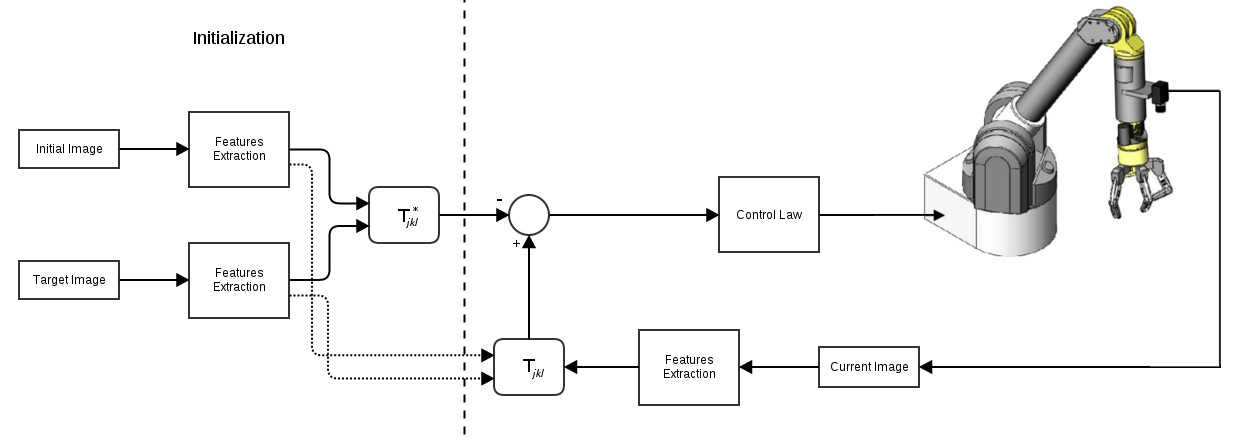
\includegraphics[width=150mm,height=70mm]{figures/vsttloop.png}
  \caption{Block diagram of the proposed Trifocal Tensor Visual Servoing loop control}
  \label{fig:vsttloop}
\end{figure}

In Figure~\ref{fig:vsttloop}, we present the block diagram explaining the proposed trifocal tensor visual servoing control loop. At initialization, the desired tensor $T_{(jkl)}^{*}$ is computed from feature correspondences across three images obtained from the three camera poses: initial pose, desired pose, and current pose being equal to the desired pose. In this method, we assume the camera intrinsic parameters are known. It means before computing the tensor from image correspondences, matching points have to be transformed to calibrated coordinates.

The current tensor $T_{(jkl)}$ is computed inside the visual servoing loop at each iteration. Then the interaction matrix is computed using the current tensor. For simplicity, we make the assumption that the initial pose is known and the interaction matrix can be computed directly. The new error value is computed along with the pseudo-inverse of the interaction matrix and fed back to the control law to compute the required velocities to drive the camera to the desired pose. The system converges and the loop is terminated when the camera reaches the desired pose. This is evaluated when the sum squared of the error reaches a value less than a defined threshold, $1 \times \e{-6}$ for example.

\chapter{Experimental Results} \label{chap:results}

In this chapter, we begin by describing the experimental setup for the proposed method we present. Then the results of applying the method on several scene configurations are presented. For each configuration we present a comparison between the ideal theoretical results obtained by computing the tensor from given known camera poses, and the practical results obtained from matching image correspondences and estimating the tensor numerically.

\section{Experimental Setup}
The proposed method was implemented in C++, and using the \texttt{ViSP} library. \texttt{ViSP} is an open-source visual servoing framework library developed by \texttt{INRIA} and written in C++ \cite{visp}. It is a modular cross platform library that allows prototyping and developing applications using visual tracking and visual servoing techniques. The implementation is divided into two main classes: Visual Servoing Manager, and Trifocal Tensor.

The Trifocal Tensor class was implemented similar to the available data types classes in \texttt{ViSP}, like Matrices and Vectors. This class is responsible for:
\begin{itemize}
  \item Storing the numerical values of the tensor.
  \item Computing the tensor using pose projection matrices.
  \item Computing the tensor using image correspondences across three images.
  \item Recovering epipoles and projection matrices.
  \item Normalizing the tensor.
  \item Computing the interaction matrix corresponding to the tensor instance.
\end{itemize}

The Visual Servoing Manager class is where the simulator, the scene, and the visual servoing task are defined. The class is responsible for:
\begin{itemize}
  \item Defining the scene configuration, the initial and desired poses.
  \item Storing different instances of the current and desired trifocal tensors.
  \item Computing the control law and velocities of the simulation camera.
  \item Plotting graphs and camera simulations showing the variation of tensor error values, computed velocities, and 3D camera end trajectories.
\end{itemize}

\begin{figure}[ht!]
\centering
\begin{adjustbox}{minipage=.9\linewidth,margin=1ex,bgcolor=black!5,margin=0.3pt,bgcolor=black!30,margin=2ex}
%\begin{mdframed}[linecolor=black!30,backgroundcolor=black!5]
  \centering
  \begin{subfigure}{.48\textwidth}
    \centering
    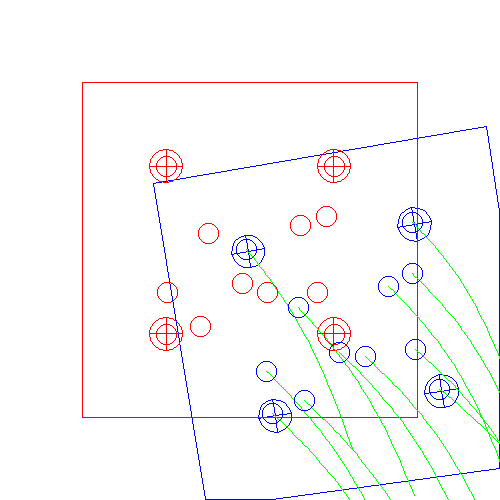
\includegraphics[width=60mm]{figures/rescamera.png}
    \caption{}
    \label{fig:rescamera}
  \end{subfigure}
  \begin{subfigure}{.48\textwidth}
    \centering
    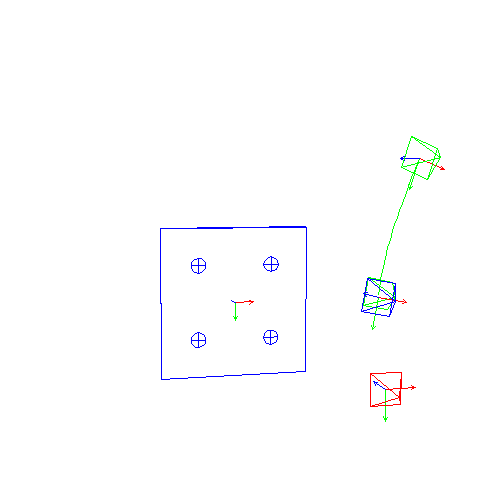
\includegraphics[width=60mm]{figures/resscene.png}
    \caption{}
    \label{fig:resscene}
  \end{subfigure}
  \caption{Experimental Setup (a) Image view with Current/Desired camera projected images plotted in blue/red, with the points trajectory in green. (b) Scene view with initial/current/desired cameras plotted in green/blue/red, with the camera trajectory in green.}
  \label{fig:ressetup}
  %\end{mdframed}
  \end{adjustbox}
\end{figure}

\newpage
The scene setup is defined with two poses for the camera: initial and desired, along with a plate object to be tracked in the scene. A trifocal tensor requires at least 7 non coplanar points for estimating a tensor. Throughout our experiments, we used two sets of 8 and 12 points. There are no much differences between the results of the two sets because we are not considering points mismatch and outliers throughout the experiments. The following results are for the set of 12 points. Throughout the results we show two different views: Image view, and Scene view. Figure \ref{fig:rescamera} shows the image view with projected current and desired camera images plotted in blue and red respectively, along with the points trajectories in green. Figure \ref{fig:resscene} shows the scene view with the position of the initial, current, and desired camera frames plotted in green, blue and red respectively. The resulting camera trajectory is plotted in green.

\section{Experiment I: Pure Translation along x-axis, y-axis}
For first experiment, we consider a pure translational motion along one axis. It's the basic test that can be done to ensure the convergence of the control loop. We consider a small translation of $0.1m$ along x-axis, then y-axis. Figure \ref{fig:ex1p} shows the results of computing the tensor using the pose.  Figure \ref{fig:ex1pvelocity} shows the evolution of the camera velocities, and Figure \ref{fig:ex1perror} shows the evolution of the trifocal tensor coefficients error. Figure \ref{fig:ex1c} shows the results of estimating the tensor through points correspondences. A translation along y-axis produces similar results.

\begin{figure}[ht!]
\begin{mdframed}[linecolor=black!30,backgroundcolor=black!5]
%\begin{adjustbox}{minipage=\linewidth,margin=1ex,bgcolor=black!5,margin=0.3pt,bgcolor=black!30,margin=2ex}
  \centering
  \begin{subfigure}{.48\linewidth}
    \centering
    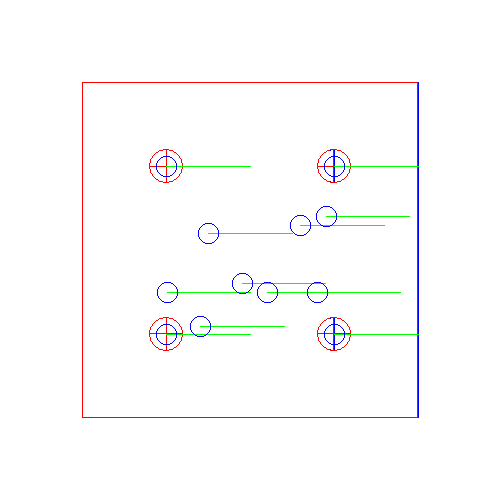
\includegraphics[width=65mm]{figures/plots/ex1pimage.png}
    \caption{}
    \label{fig:ex1pimage}
  \end{subfigure}
  \begin{subfigure}{.48\linewidth}
    \centering
    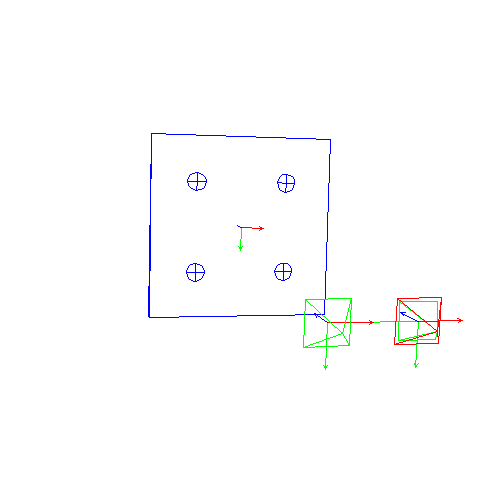
\includegraphics[width=65mm]{figures/plots/ex1pscene.png}
    \caption{}
    \label{fig:ex1pscene}
  \end{subfigure}
  \\
  \begin{subfigure}{.48\linewidth}
    \centering
    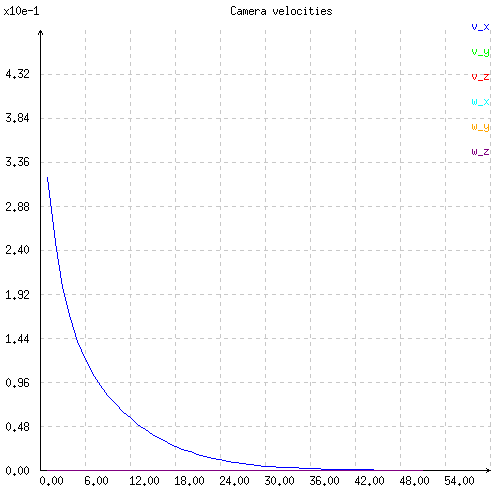
\includegraphics[width=65mm]{figures/plots/ex1pvelocity.png}
    \caption{}
    \label{fig:ex1pvelocity}
  \end{subfigure}
  \begin{subfigure}{.48\linewidth}
    \centering
    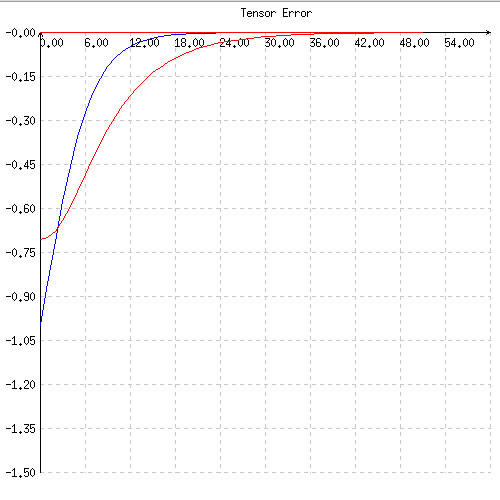
\includegraphics[width=65mm]{figures/plots/ex1perror.png}
    \caption{}
    \label{fig:ex1perror}
  \end{subfigure}
  \caption{Translation along x-axis using tensor from poses. (a) Image view. (b) Scene view. (c) Camera velocities. (d) Tensor coefficients error.}
  \label{fig:ex1p}
\end{mdframed}
%\end{adjustbox}
\end{figure}

\begin{figure}[ht!]
\centering
\begin{mdframed}[linecolor=black!30,backgroundcolor=black!5]
%\begin{adjustbox}{minipage=.8\linewidth,margin=1ex,bgcolor=black!5,margin=0.3pt,bgcolor=black!30,margin=2ex}
  \centering
  \begin{subfigure}{.48\textwidth}
    \centering
    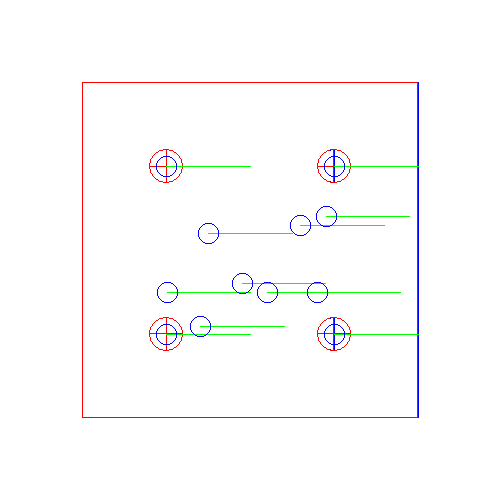
\includegraphics[width=65mm]{figures/plots/ex1pimage.png}
    \caption{}
    \label{fig:ex1cimage}
  \end{subfigure}
  \begin{subfigure}{.48\textwidth}
    \centering
    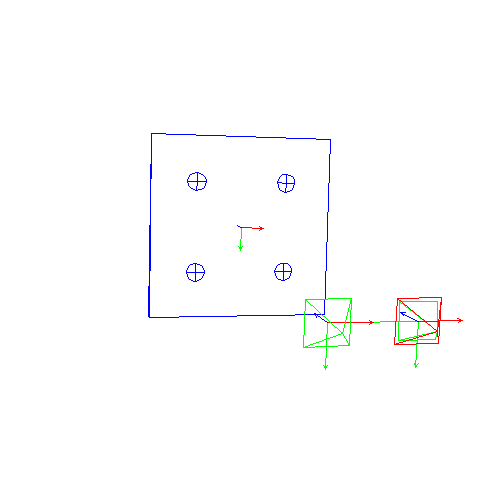
\includegraphics[width=65mm]{figures/plots/ex1pscene.png}
    \caption{}
    \label{fig:ex1cscene}
  \end{subfigure}
  \\
  \begin{subfigure}{.48\textwidth}
    \centering
    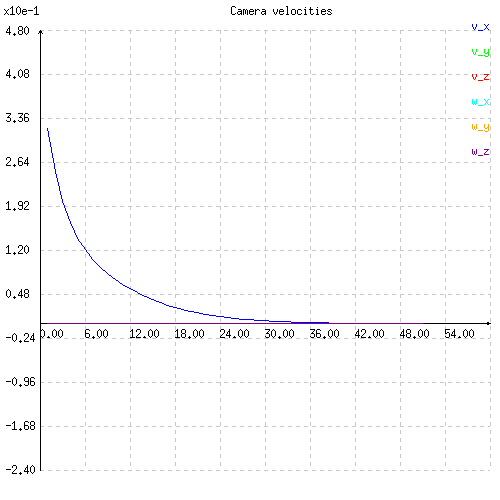
\includegraphics[width=65mm]{figures/plots/ex1cvelocity.png}
    \caption{}
    \label{fig:ex1cvelocity}
  \end{subfigure}
  \begin{subfigure}{.48\textwidth}
    \centering
    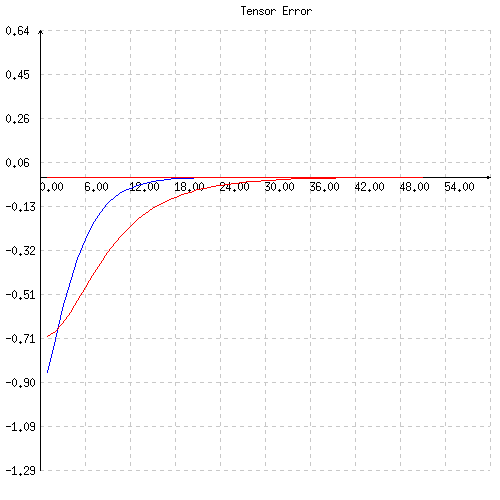
\includegraphics[width=65mm]{figures/plots/ex1cerror.png}
    \caption{}
    \label{fig:ex1cerror}
  \end{subfigure}
  \caption{Translation along x-axis using estimated tensor. (a) Image view. (b) Scene view. (c) Camera velocities. (d) Tensor coefficients error.}
  \label{fig:ex1c}
\end{mdframed}
%\end{adjustbox}
\end{figure}
\clearpage

The system behaviour in both cases is identical. We observe the camera trajectory is linear, which is satisfactory. However, the error is not exactly exponentially decreasing. Several tests were conducted to analyse the source of this behaviour, and it was found that using a subset of tensor coefficients for computing the error and the interaction matrix leads to a perfect exponentially decreasing error. A subset was chosen experimentally to handle this specific configuration, but for different subsets are then required for different configurations. The problem of subset selection is discussed in details in \ref{sec:futurework}. Figure \ref{fig:ex1comparison} shows a comparison between the error plots using all the tensor coefficients and using a subset of them.

\begin{figure}[ht!]
\centering
\begin{adjustbox}{minipage=.9\linewidth,margin=1ex,bgcolor=black!5,margin=0.3pt,bgcolor=black!30,margin=2ex}
  \centering
  \begin{subfigure}{.48\textwidth}
    \centering
    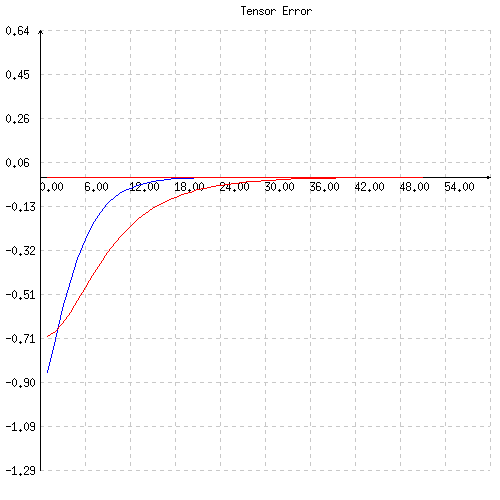
\includegraphics[width=60mm]{figures/plots/ex1cerror.png}
    \caption{}
    \label{fig:ex1comparisona}
  \end{subfigure}
  \begin{subfigure}{.48\textwidth}
    \centering
    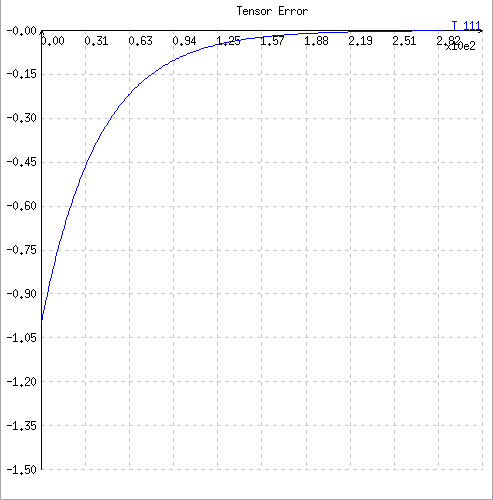
\includegraphics[width=60mm]{figures/plots/ex1subset.png}
    \caption{}
    \label{fig:ex1comparisonb}
  \end{subfigure}
  \caption{Comparison between tensor coefficients error when (a) using all tensor coefficients (b) using a subset of tensor coefficients.}
  \label{fig:ex1comparison}
  \end{adjustbox}
\end{figure}

\section{Experiment II: Pure Translation along z-axis}
Motion along the z-axis is usually more challenging than xyz motion in the IBVS approach. This is due to poor motion resolvability when the camera moves towards the feature points \cite{nelson1996vision}. On the contrary, using the trifocal tensor features this motion is not different than other types of motions. Figure \ref{fig:ex2p} and Figure \ref{fig:ex2c} show the results for the pose and estimated tensors respectively. Like a simple translation along x-axis or y-axis, a translation along z-axis also suffers the problem of selecting a subset of tensor coefficients.

\begin{figure}[ht!]
\begin{mdframed}[linecolor=black!30,backgroundcolor=black!5]
%\begin{adjustbox}{minipage=\linewidth,margin=1ex,bgcolor=black!5,margin=0.3pt,bgcolor=black!30,margin=2ex}
  \centering
  \begin{subfigure}{.48\linewidth}
    \centering
    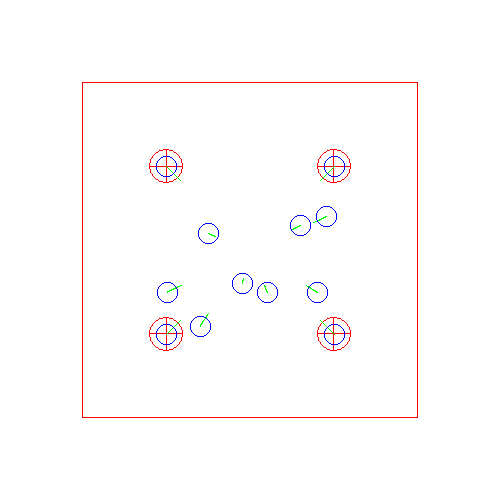
\includegraphics[width=65mm]{figures/plots/ex2pimage.png}
    \caption{}
    \label{fig:ex2pimage}
  \end{subfigure}
  \begin{subfigure}{.48\linewidth}
    \centering
    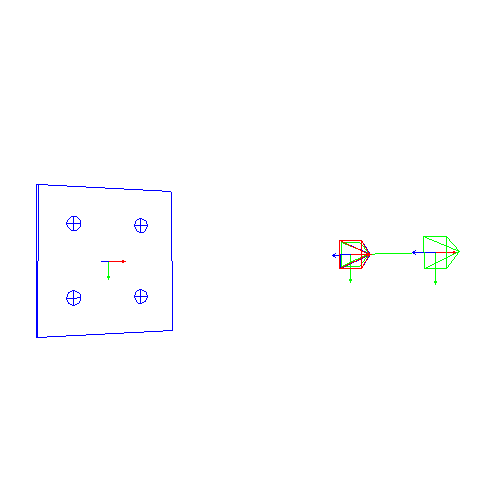
\includegraphics[width=65mm]{figures/plots/ex2pscene.png}
    \caption{}
    \label{fig:ex2pscene}
  \end{subfigure}
  \\
  \begin{subfigure}{.48\linewidth}
    \centering
    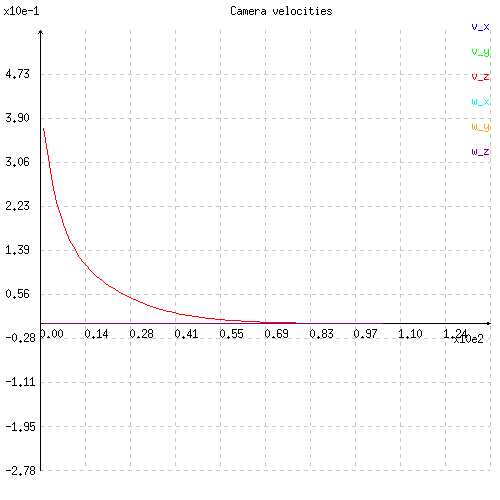
\includegraphics[width=65mm]{figures/plots/ex2pvelocity.png}
    \caption{}
    \label{fig:ex2pvelocity}
  \end{subfigure}
  \begin{subfigure}{.48\linewidth}
    \centering
    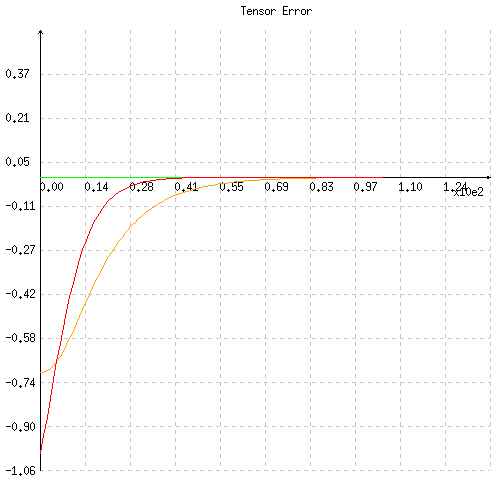
\includegraphics[width=65mm]{figures/plots/ex2perror.png}
    \caption{}
    \label{fig:ex2perror}
  \end{subfigure}
  \caption{Translation along z-axis using tensor from poses. (a) Image view. (b) Scene view. (c) Camera velocities. (d) Tensor coefficients error.}
  \label{fig:ex2p}
\end{mdframed}
%\end{adjustbox}
\end{figure}

\begin{figure}[ht!]
\centering
\begin{mdframed}[linecolor=black!30,backgroundcolor=black!5]
%\begin{adjustbox}{minipage=.8\linewidth,margin=1ex,bgcolor=black!5,margin=0.3pt,bgcolor=black!30,margin=2ex}
  \centering
  \begin{subfigure}{.48\textwidth}
    \centering
    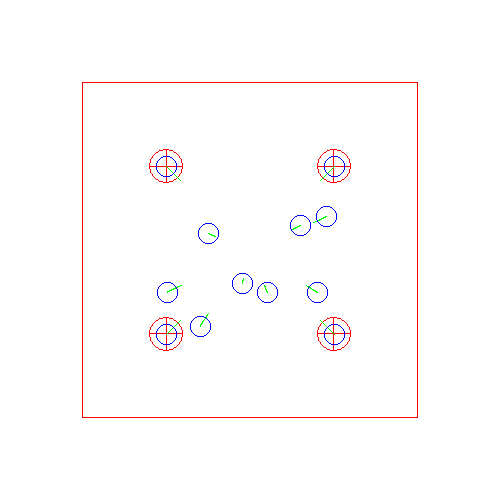
\includegraphics[width=65mm]{figures/plots/ex2pimage.png}
    \caption{}
    \label{fig:ex2cimage}
  \end{subfigure}
  \begin{subfigure}{.48\textwidth}
    \centering
    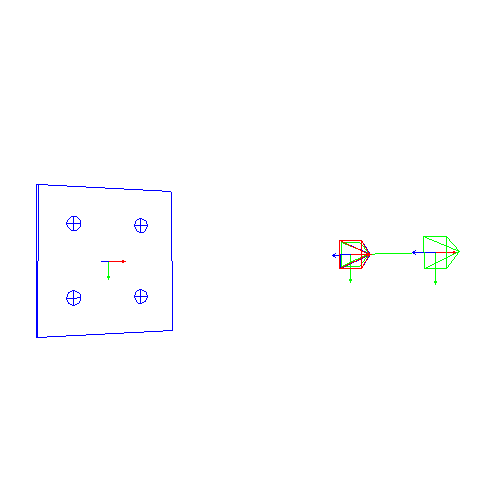
\includegraphics[width=65mm]{figures/plots/ex2pscene.png}
    \caption{}
    \label{fig:ex2cscene}
  \end{subfigure}
  \\
  \begin{subfigure}{.48\textwidth}
    \centering
    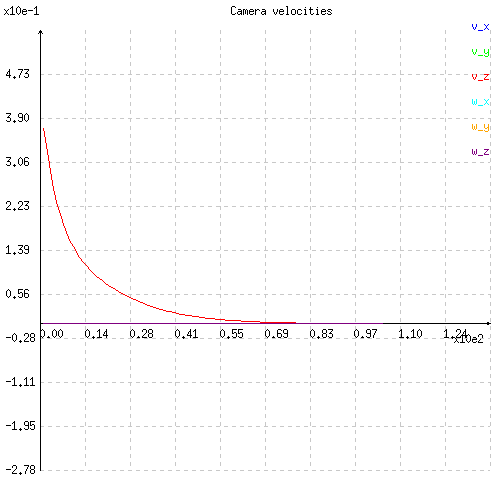
\includegraphics[width=65mm]{figures/plots/ex2cvelocity.png}
    \caption{}
    \label{fig:ex2cvelocity}
  \end{subfigure}
  \begin{subfigure}{.48\textwidth}
    \centering
    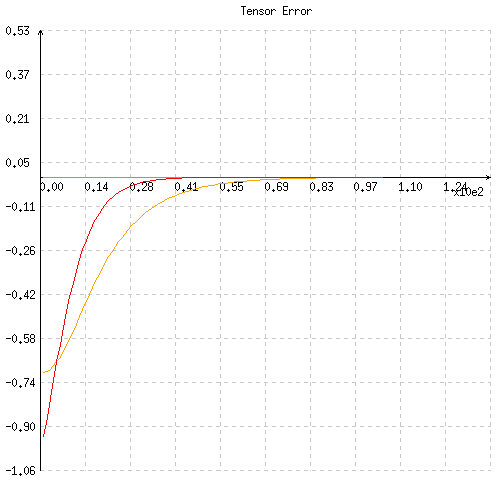
\includegraphics[width=65mm]{figures/plots/ex2cerror.png}
    \caption{}
    \label{fig:ex2cerror}
  \end{subfigure}
  \caption{Translation along z-axis using estimated tensor. (a) Image view. (b) Scene view. (c) Camera velocities. (d) Tensor coefficients error.}
  \label{fig:ex2c}
\end{mdframed}
%\end{adjustbox}
\end{figure}

\section{Experiment III: Translation along xyz-axes}
Now we consider a motion along the 3 x,y, and z axes. From Figure \ref{fig:ex3perror} and \ref{fig:ex3cerror}, we observe the tensor error is not behaving as a desired exponentially decreasing function. However, the camera trajectory is still linear, which is expected and satisfactory.

\begin{figure}[ht!]
\begin{mdframed}[linecolor=black!30,backgroundcolor=black!5]
%\begin{adjustbox}{minipage=\linewidth,margin=1ex,bgcolor=black!5,margin=0.3pt,bgcolor=black!30,margin=2ex}
  \centering
  \begin{subfigure}{.48\linewidth}
    \centering
    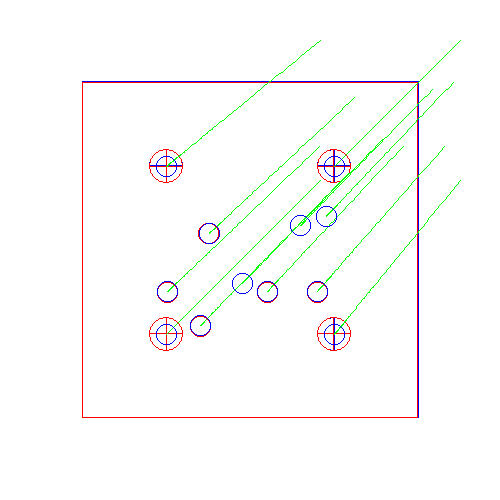
\includegraphics[width=65mm]{figures/plots/ex3pimage.png}
    \caption{}
    \label{fig:ex3pimage}
  \end{subfigure}
  \begin{subfigure}{.48\linewidth}
    \centering
    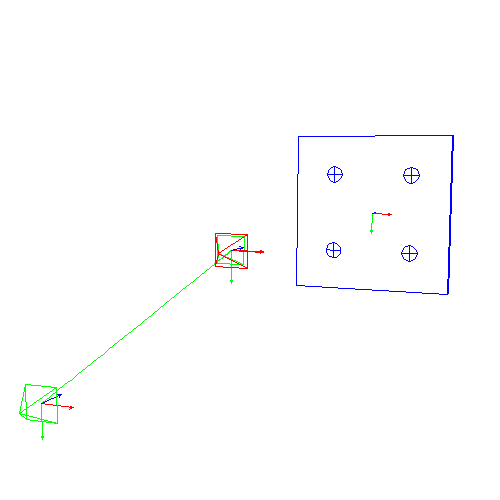
\includegraphics[width=65mm]{figures/plots/ex3pscene.png}
    \caption{}
    \label{fig:ex3pscene}
  \end{subfigure}
  \\
  \begin{subfigure}{.48\linewidth}
    \centering
    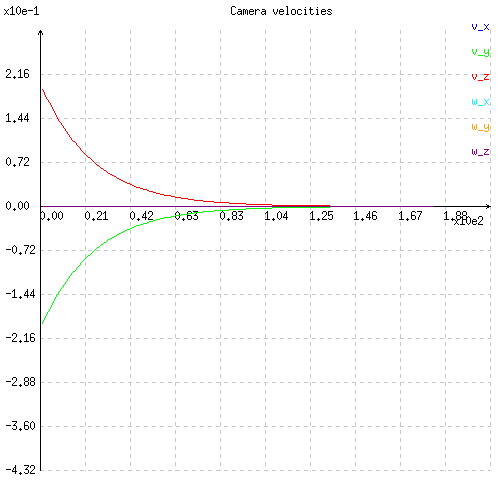
\includegraphics[width=65mm]{figures/plots/ex3pvelocity.png}
    \caption{}
    \label{fig:ex3pvelocity}
  \end{subfigure}
  \begin{subfigure}{.48\linewidth}
    \centering
    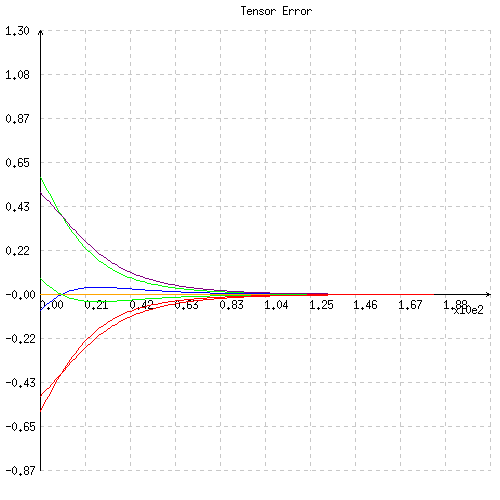
\includegraphics[width=65mm]{figures/plots/ex3perror.png}
    \caption{}
    \label{fig:ex3perror}
  \end{subfigure}
  \caption{Translation along xyz-axes using tensor from poses. (a) Image view. (b) Scene view. (c) Camera velocities. (d) Tensor coefficients error.}
  \label{fig:ex3p}
\end{mdframed}
%\end{adjustbox}
\end{figure}

\begin{figure}[ht!]
\centering
\begin{mdframed}[linecolor=black!30,backgroundcolor=black!5]
%\begin{adjustbox}{minipage=.8\linewidth,margin=1ex,bgcolor=black!5,margin=0.3pt,bgcolor=black!30,margin=2ex}
  \centering
  \begin{subfigure}{.48\textwidth}
    \centering
    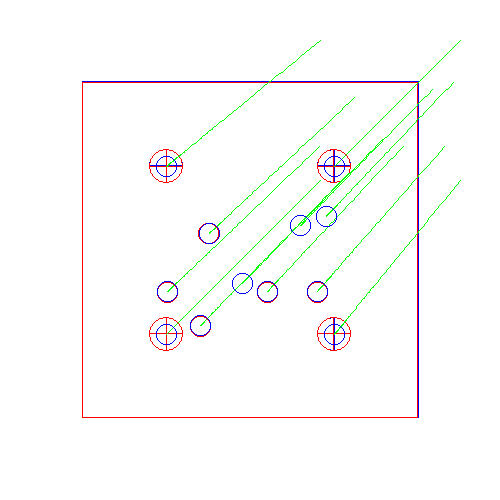
\includegraphics[width=65mm]{figures/plots/ex3cimage.png}
    \caption{}
    \label{fig:ex3cimage}
  \end{subfigure}
  \begin{subfigure}{.48\textwidth}
    \centering
    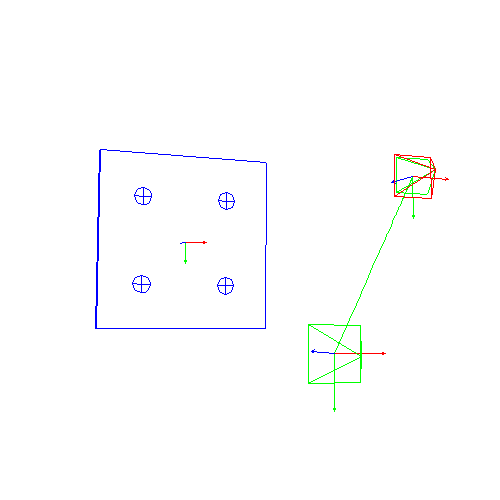
\includegraphics[width=65mm]{figures/plots/ex3cscene.png}
    \caption{}
    \label{fig:ex3cscene}
  \end{subfigure}
  \\
  \begin{subfigure}{.48\textwidth}
    \centering
    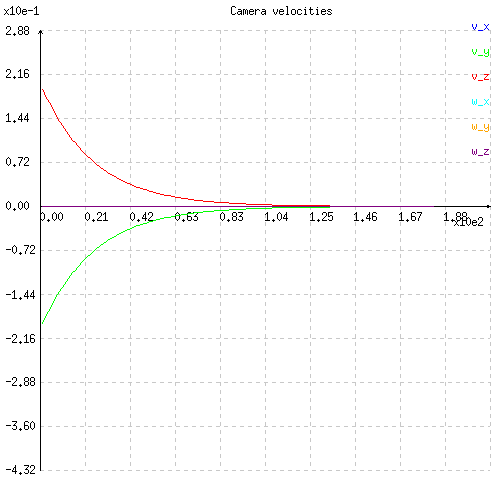
\includegraphics[width=65mm]{figures/plots/ex3cvelocity.png}
    \caption{}
    \label{fig:ex3cvelocity}
  \end{subfigure}
  \begin{subfigure}{.48\textwidth}
    \centering
    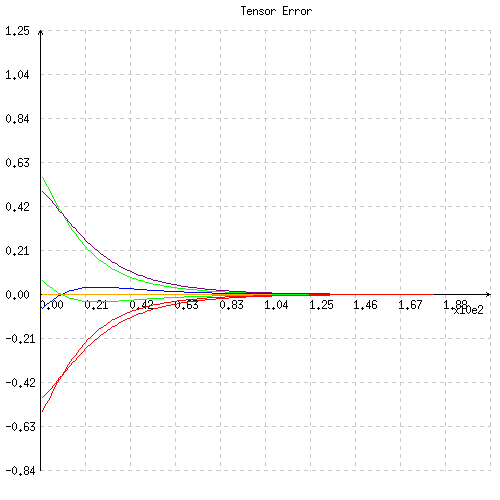
\includegraphics[width=65mm]{figures/plots/ex3cerror.png}
    \caption{}
    \label{fig:ex3cerror}
  \end{subfigure}
  \caption{Translation along xyz-axes using estimated tensor. (a) Image view. (b) Scene view. (c) Camera velocities. (d) Tensor coefficients error.}
  \label{fig:ex3c}
\end{mdframed}
%\end{adjustbox}
\end{figure}

\section{Experiment IV: Large rotation around z-axis}
One of the most challenging IBVS configurations is the $180$\textdegree rotation around the z-axis \cite{chaumette2006visual}\cite{chaumette1998potential}. This is due to the nature of the image-based control law which makes the camera retreat from the object instead of rotating around the z-axis. It is important to evaluate the visual servoing method for large z-axis rotations, close to $180$\textdegree.

Here we consider a translation of $1m$ and a $170$\textdegree rotation. As we can observe in Figure \ref{fig:ex4p} and Figure \ref{fig:ex4c}, the retreat problem didn't occur. The image trajectories follow a spiral motion, which is exactly as expected due to the linear motion for the translation, and the rotational motion for the rotation.

\begin{figure}[ht!]
\begin{mdframed}[linecolor=black!30,backgroundcolor=black!5]
%\begin{adjustbox}{minipage=\linewidth,margin=1ex,bgcolor=black!5,margin=0.3pt,bgcolor=black!30,margin=2ex}
  \centering
  \begin{subfigure}{.48\linewidth}
    \centering
    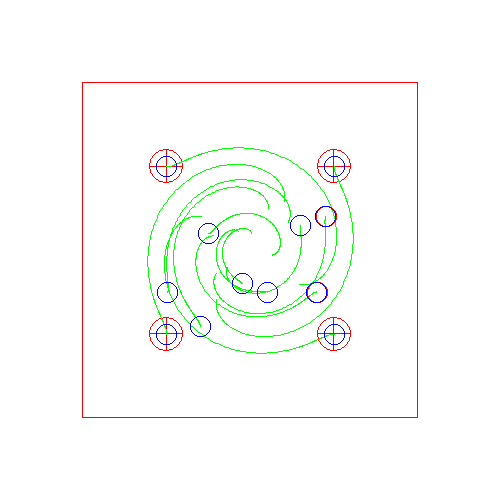
\includegraphics[width=65mm]{figures/plots/ex4pimage.png}
    \caption{}
    \label{fig:ex4pimage}
  \end{subfigure}
  \begin{subfigure}{.48\linewidth}
    \centering
    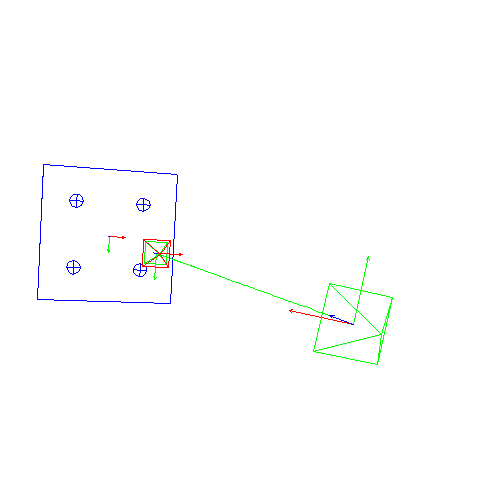
\includegraphics[width=65mm]{figures/plots/ex4pscene.png}
    \caption{}
    \label{fig:ex4pscene}
  \end{subfigure}
  \\
  \begin{subfigure}{.48\linewidth}
    \centering
    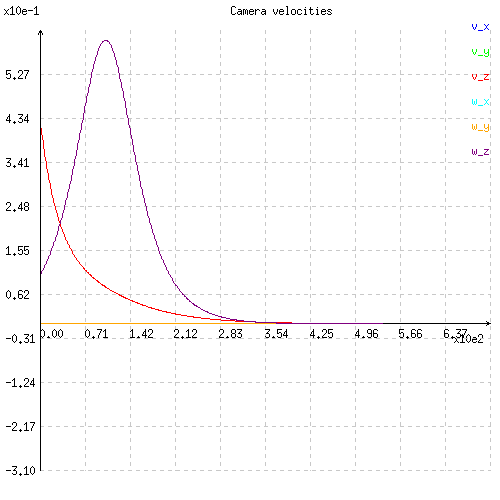
\includegraphics[width=65mm]{figures/plots/ex4pvelocity.png}
    \caption{}
    \label{fig:ex4pvelocity}
  \end{subfigure}
  \begin{subfigure}{.48\linewidth}
    \centering
    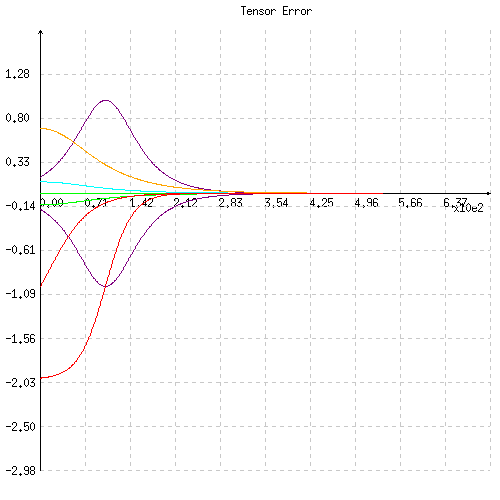
\includegraphics[width=65mm]{figures/plots/ex4perror.png}
    \caption{}
    \label{fig:ex4perror}
  \end{subfigure}
  \caption{Translation and large rotation along z-axis using tensor from poses. (a) Image view. (b) Scene view. (c) Camera velocities. (d) Tensor coefficients error.}
  \label{fig:ex4p}
\end{mdframed}
%\end{adjustbox}
\end{figure}

\begin{figure}[ht!]
\centering
\begin{mdframed}[linecolor=black!30,backgroundcolor=black!5]
%\begin{adjustbox}{minipage=.8\linewidth,margin=1ex,bgcolor=black!5,margin=0.3pt,bgcolor=black!30,margin=2ex}
  \centering
  \begin{subfigure}{.48\textwidth}
    \centering
    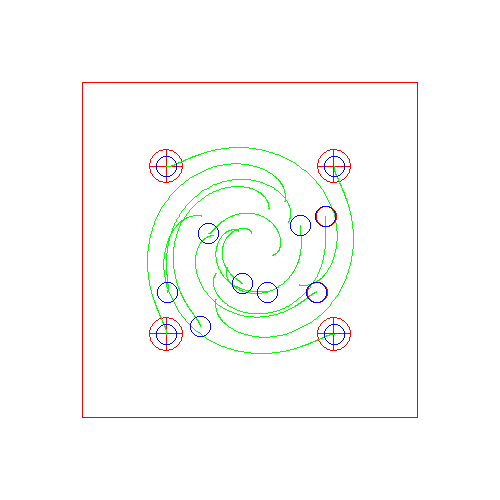
\includegraphics[width=65mm]{figures/plots/ex4cimage.png}
    \caption{}
    \label{fig:ex4cimage}
  \end{subfigure}
  \begin{subfigure}{.48\textwidth}
    \centering
    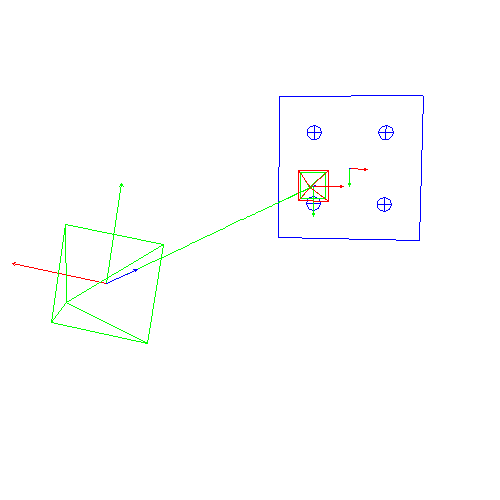
\includegraphics[width=65mm]{figures/plots/ex4cscene.png}
    \caption{}
    \label{fig:ex4cscene}
  \end{subfigure}
  \\
  \begin{subfigure}{.48\textwidth}
    \centering
    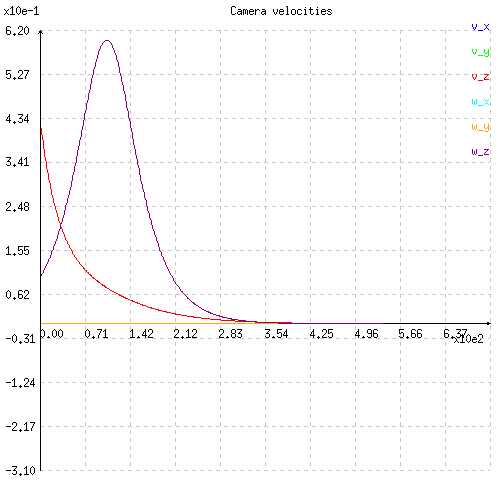
\includegraphics[width=65mm]{figures/plots/ex4cvelocity.png}
    \caption{}
    \label{fig:ex4cvelocity}
  \end{subfigure}
  \begin{subfigure}{.48\textwidth}
    \centering
    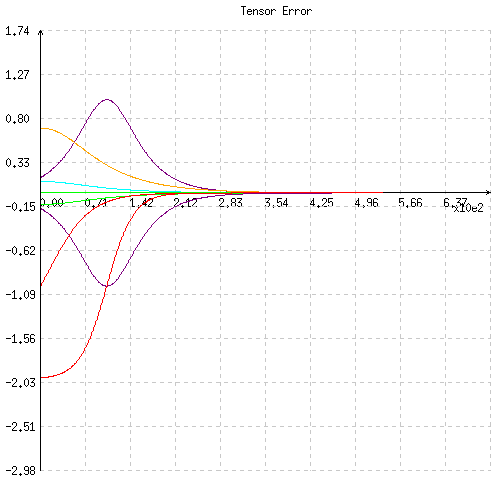
\includegraphics[width=65mm]{figures/plots/ex4cerror.png}
    \caption{}
    \label{fig:ex4cerror}
  \end{subfigure}
  \caption{Translation and large rotation along z-axis using estimated tensor. (a) Image view. (b) Scene view. (c) Camera velocities. (d) Tensor coefficients error.}
  \label{fig:ex4c}
\end{mdframed}
%\end{adjustbox}
\end{figure}

\section{Experiment V: Generic Motion}
In this experiment, we choose a generic camera motion: translations of $0.25m, -0.3m, 0.2m$, and rotations of $10\text{\textdegree}, -20\text{\textdegree}, 5\text{\textdegree}$ along x,y, and z axes respectively. The results in Figures \ref{fig:ex5p} and \ref{fig:ex5c} show smooth camera and image trajectories. However, comparing the two Figures \ref{fig:ex5pvelocity} and \ref{fig:ex5cvelocity}, we notice small oscillations in the camera velocities initially. Lopez-Nicolas \cite{lopez2010visual} mentioned similar oscillations due to noise during image points extraction and matching. Although in our case we omit points mismatch and outliers, but this behaviour is most likely due to small numerical error in the trifocal tensor estimation, as the pose tensor doesn't produce similar oscillations.

\begin{figure}[ht!]
\begin{mdframed}[linecolor=black!30,backgroundcolor=black!5]
%\begin{adjustbox}{minipage=\linewidth,margin=1ex,bgcolor=black!5,margin=0.3pt,bgcolor=black!30,margin=2ex}
  \centering
  \begin{subfigure}{.48\linewidth}
    \centering
    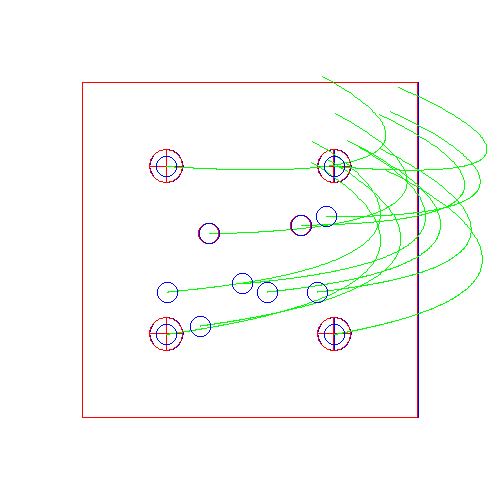
\includegraphics[width=65mm]{figures/plots/ex5pimage.png}
    \caption{}
    \label{fig:ex5pimage}
  \end{subfigure}
  \begin{subfigure}{.48\linewidth}
    \centering
    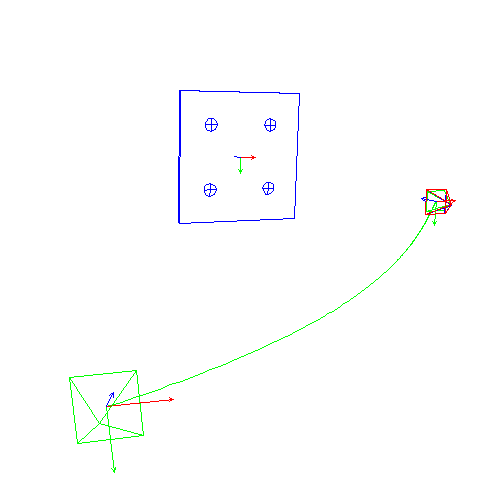
\includegraphics[width=65mm]{figures/plots/ex5pscene.png}
    \caption{}
    \label{fig:ex5pscene}
  \end{subfigure}
  \\
  \begin{subfigure}{.48\linewidth}
    \centering
    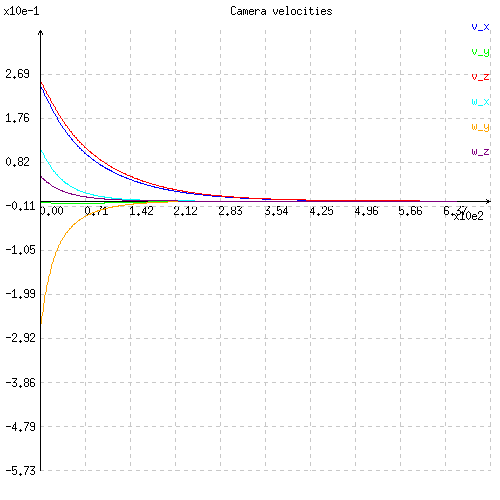
\includegraphics[width=65mm]{figures/plots/ex5pvelocity.png}
    \caption{}
    \label{fig:ex5pvelocity}
  \end{subfigure}
  \begin{subfigure}{.48\linewidth}
    \centering
    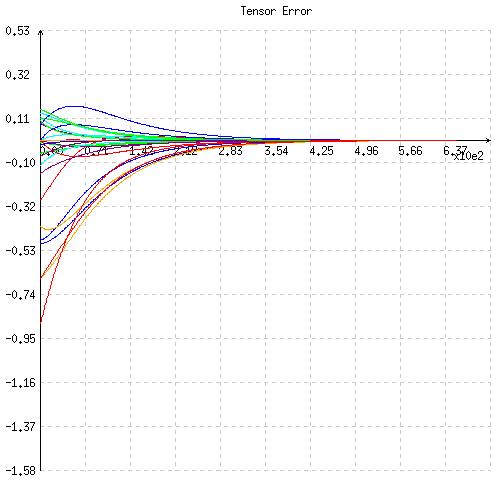
\includegraphics[width=65mm]{figures/plots/ex5perror.png}
    \caption{}
    \label{fig:ex5perror}
  \end{subfigure}
  \caption{Generic motion using tensor from poses. (a) Image view. (b) Scene view. (c) Camera velocities. (d) Tensor coefficients error.}
  \label{fig:ex5p}
\end{mdframed}
%\end{adjustbox}
\end{figure}

\begin{figure}[ht!]
\centering
\begin{mdframed}[linecolor=black!30,backgroundcolor=black!5]
%\begin{adjustbox}{minipage=.8\linewidth,margin=1ex,bgcolor=black!5,margin=0.3pt,bgcolor=black!30,margin=2ex}
  \centering
  \begin{subfigure}{.48\textwidth}
    \centering
    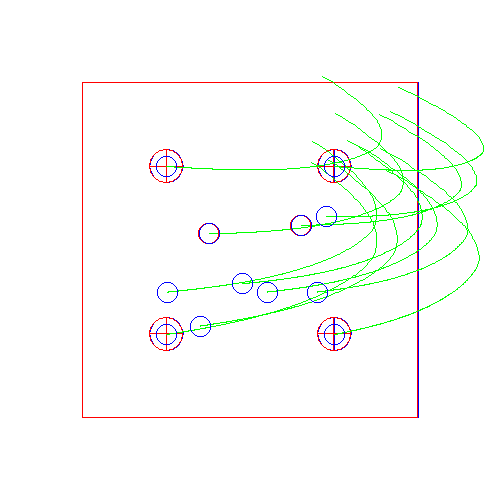
\includegraphics[width=65mm]{figures/plots/ex5cimage.png}
    \caption{}
    \label{fig:ex5cimage}
  \end{subfigure}
  \begin{subfigure}{.48\textwidth}
    \centering
    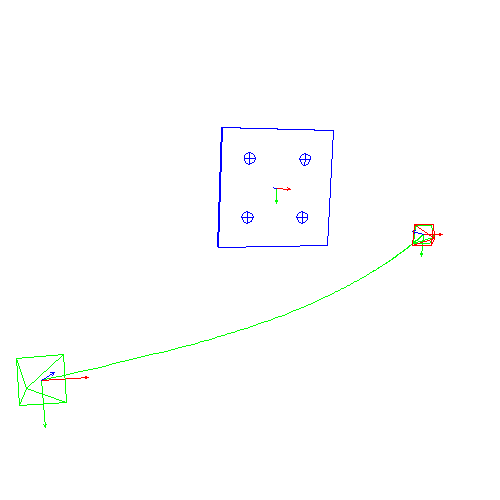
\includegraphics[width=65mm]{figures/plots/ex5cscene.png}
    \caption{}
    \label{fig:ex5cscene}
  \end{subfigure}
  \\
  \begin{subfigure}{.48\textwidth}
    \centering
    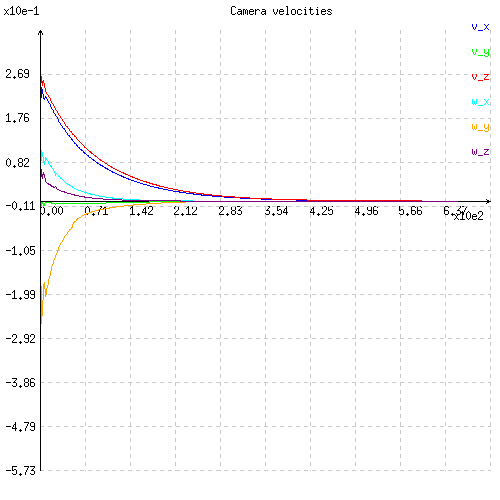
\includegraphics[width=65mm]{figures/plots/ex5cvelocity.png}
    \caption{}
    \label{fig:ex5cvelocity}
  \end{subfigure}
  \begin{subfigure}{.48\textwidth}
    \centering
    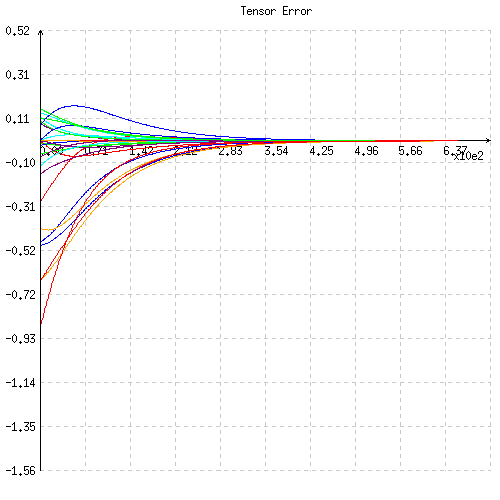
\includegraphics[width=65mm]{figures/plots/ex5cerror.png}
    \caption{}
    \label{fig:ex5cerror}
  \end{subfigure}
  \caption{Generic motion using estimated tensor. (a) Image view. (b) Scene view. (c) Camera velocities. (d) Tensor coefficients error.}
  \label{fig:ex5c}
\end{mdframed}
%\end{adjustbox}
\end{figure}

\chapter{Conclusion and Future Work} \label{chap:conclusion}

\section{Conclusion}
Visual Servoing is a growing active field of research. Recent advances in robotics and computer vision domains has led to the emergence of this vision-based closed loop control methods to control a robot manipulator or a mobile robot through vision acquired by a camera. Many works have studied closing the control loop over visual features computed either from the image space or the estimated 3D pose of the scene. Few works studied using stereo-vision geometry, and up until recently only a couple of works studied using the trifocal tensor into the visual servoing control loop.

An approach to incorporate the trifocal tensor estimated from the three-views geometry into the visual servoing control loop task has been presented in this work. This approach presents a generalized 6-DOF visual servoing task, with the control loop being closed over projective measures, namely the trifocal tensor coefficients. To the best of our knowledge, this approach is the first to propose a fully analytical design for a visual servoing task based on the trifocal tensor. Previous works either provided an analytical approach for a 3-DOF non-holonomic mobile robot, or provided a full 6-DOF approach but with an interaction matrix estimated numerically rather than analytically.

The experiments showed that this approach is working practically with very satisfactory results. In addition, this approach does not suffer from some of the problems existing in IBVS methods as like the retreat problem.

\section{Future Work}\label{sec:futurework}
\subsection{Using A Subset of the Trifocal Tensor Coefficients}
As presented in \ref{chap:results}, it was found that using all the trifocal tensor coefficients inside the visual servoing loop does not produce the best results in terms of perfectly exponentially decreasing tensor error values. Thus, an automatic optimality selection criteria is needed to dynamically choose the most relevant tensor coefficients. For example, the singular value decomposition of the interaction matrix can reveal which degrees of freedom are most apparent. By selecting features and designing controllers that maximize these measures, the performance of the visual servoing system can be improved. These concepts has been discussed in details in \cite{chaumette2007visual}, \cite{538976} and \cite{611333}.
\vspace{-1em}
\subsection{Stability Analysis}
Simulation and practical experiments are not enough for judging the proposed method. We need to prove the existence of only one equilibrium state at the desired pose location. The analysis of the control law can be studied using Lyapunov stability analysis method \cite{spong2006robot}.
\vspace{-1em}
\subsection{Estimating The Initial Pose}
We observe in \eqref{eq:interactionmatrixnormalized} that the interaction matrix depends on the knowledge of the initial camera pose. In our experiments, we made an assumption that the initial pose is known from the setup of the simulation. Practically, this information might not be available, and the initial pose needs to be estimated. The initial pose can be retrieved by computing the equivalent projection matrix for the estimated trifocal tensor as shown in~\ref{sub:recovering_projection_matrices}. However, one potential issue is that the estimation will be up to a scale value and not the real value. This scale problem needs to be addressed properly during the tensor normalization step to avoid the scale effects on computing the correct values for the interaction matrix.
\vspace{-1em}
\subsection{Uncalibrated Camera}
The current method assumes the cameras have already been calibrated before-hand. Practically, this may not be the case, so we need to extend the method to cover partially or totally uncalibrated cameras. The introduction of the camera intrinsic parameters matrix $K$ into the formulas, will affect the obtained tensor computation, and hence, the corresponding interaction matrix.

%\appendix
%\chapter{The first appendix}
If you need to add any appendix, do it here...
 Etc.


%   this is for BibTeX.  remove if you plan to write the references in the document
\bibliographystyle{IEEEtran}
\nocite{*}
\bibliography{tex/refs}


%adds the bibliography to the table of contents
\addcontentsline{toc}{chapter}
         {\protect\numberline{Bibliography\hspace{-96pt}}}

\end{document}
